% !Mode:: "Tex:UTF-8"

\section{Variables aleatorias.}\label{sec:variablesAletorias}

\subsection{¿Qué son las variables aleatorias?}
\label{Cap04:subsec:QueSonVariablesAleatorias}

Hemos visto que cada suceso $A$ del espacio muestral $\Omega$ tiene asociado un valor $P(A)$ de la función probabilidad. Y sabemos que los valores de la función probabilidad son valores positivos, comprendidos entre $0$ y $1$. La idea de variable aleatoria es similar, pero generaliza este concepto, porque a menudo querremos asociar otros valores numéricos con los resultados de un experimento aleatorio.
\begin{Ejemplo}
\label{cap04:ejem:VariableAleatoriaSumaDosDados}
    Quizá uno de los ejemplos más sencillos sea lo que ocurre cuando lanzamos dos dados, y nos fijamos en la suma de los valores obtenidos. Esa suma es siempre un número del 2 al 12, y es perfectamente legítimo hacer preguntas como ¿cuál es la probabilidad de que  la suma valga $7$? Para responder a esa pregunta, iríamos al espacio muestral (formado por 36 resultados posibles), veríamos el valor de la suma en cada uno de ellos, para localizar aquellos en que la suma vale $7$. Así obtendríamos un suceso aleatorio $A=\{(1,6),(2,5),(3,4),(4,3),(5,2),(6,1)\}$, cuya probabilidad es $6/36$. De hecho podemos
    repetir lo mismo para cada uno de los posibles valores de la suma. Se obtiene la Tabla \ref{cap04:tabla:probabilidadSumaDados}, que vamos a llamar la {\sf tabla de densidad} de probabilidad de la variable suma.\qed
    \begin{table}[ht]
    \begin{center}
    {\small
    \begin{tabular}[t]{|c|c|c|c|c|c|c|c|c|c|c|c|}
    \hline
    \begin{minipage}{2cm}
    \rule{0cm}{0.7cm}{\em Valor de\\ la suma:\\[2mm]}
    \end{minipage}
    &2&3&4&5&6&7&8&9&10&11&12\\
    \hline
    \begin{minipage}{2cm}
    \rule{0cm}{1cm}{\em Probabilidad\\
    de ese valor:}
    \end{minipage}
    &$\dfrac{1}{36}$&$\dfrac{2}{36}$&$\dfrac{3}{36}$&$\dfrac{4}{36}$&$\dfrac{5}{36}$&$\dfrac{6}{36}$&$\dfrac{5}{36}$&$\dfrac{4}{36}$&$\dfrac{3}{36}$&$\dfrac{2}{36}$&$\dfrac{1}{36}$\\
    &&&&&&&&&&&\\
    \hline
    \end{tabular}
    }
    \caption{Tabla de densidad de probabilidad de las posibles sumas, al lanzar dos dados}
    \label{cap04:tabla:probabilidadSumaDados}
    \end{center}
    \end{table}
\end{Ejemplo}
Vamos ahora a ver otro ejemplo, en este caso inspirado en los problemas de probabilidad geométrica.
\begin{Ejemplo}\label{ejem:ProbabilidadGeometricaSubconjuntosCirculo}
    Consideremos un círculo $C$ centrado en el origen y de radio 1. El espacio muestral $\Omega$ está formado por todos los subconjuntos\footnote{Subconjuntos que no sean excesivamente ``raros'', en el sentido que ya hemos discutido.} de puntos de $C$. Y la probabilidad de un subconjunto $A$ se define así:
    \[P(A)=\mbox{área de }A.\]
    Consideremos ahora la variable $X(x,y)=x$, que a cada punto del círculo le asocia su coordenada $x$. En este caso la coordenada $x$ toma cualquier valor real entre $-1$ y $1$. Y si preguntamos {``¿cuál es la probabilidad de que tome por ejemplo el valor $1/2$?''}, la respuesta es $0$. Porque los puntos del círculo donde toma ese valor forman un segmento (una cuerda del círculo), y el segmento tiene área $0$. Las cosas cambian si preguntamos {``¿cuál es la probabilidad de que la coordenada $x$ esté entre $0$ y $1/2$?''} En este caso, como muestra la Figura \ref{cap04:fig:EjemploVariableAleatoriaContinua}
    \begin{figure}[h]
	\centering
	\begin{enColor}
    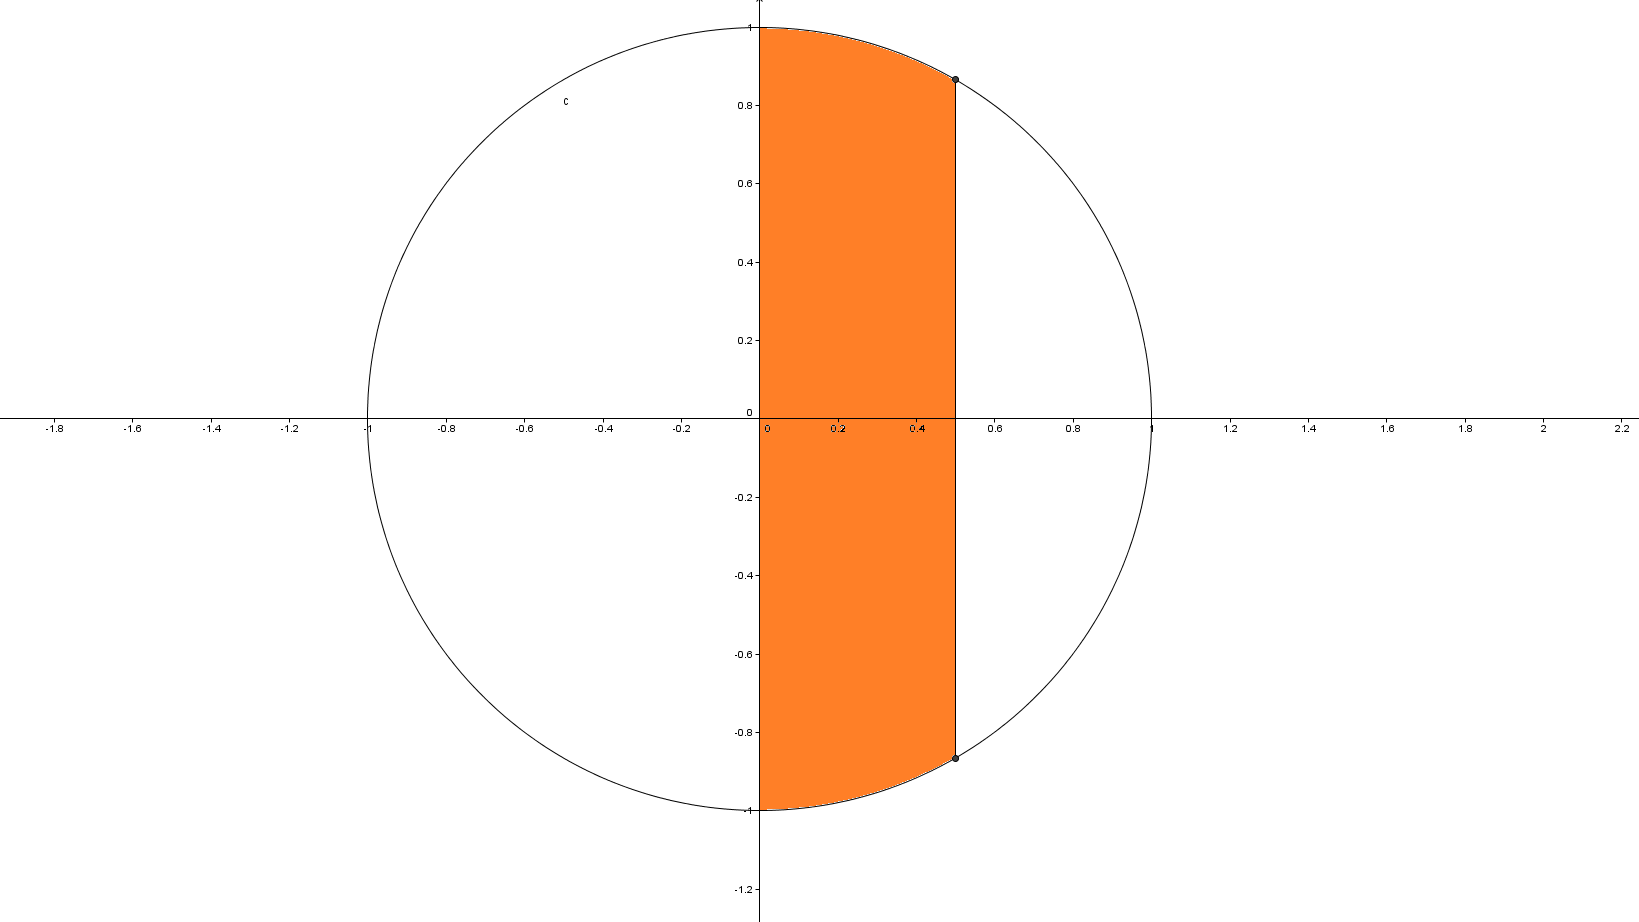
\includegraphics[height=7cm]{../fig/Cap04-Figura01-VariableAleatoriaContinua.png}
	\end{enColor}
	\begin{bn}
    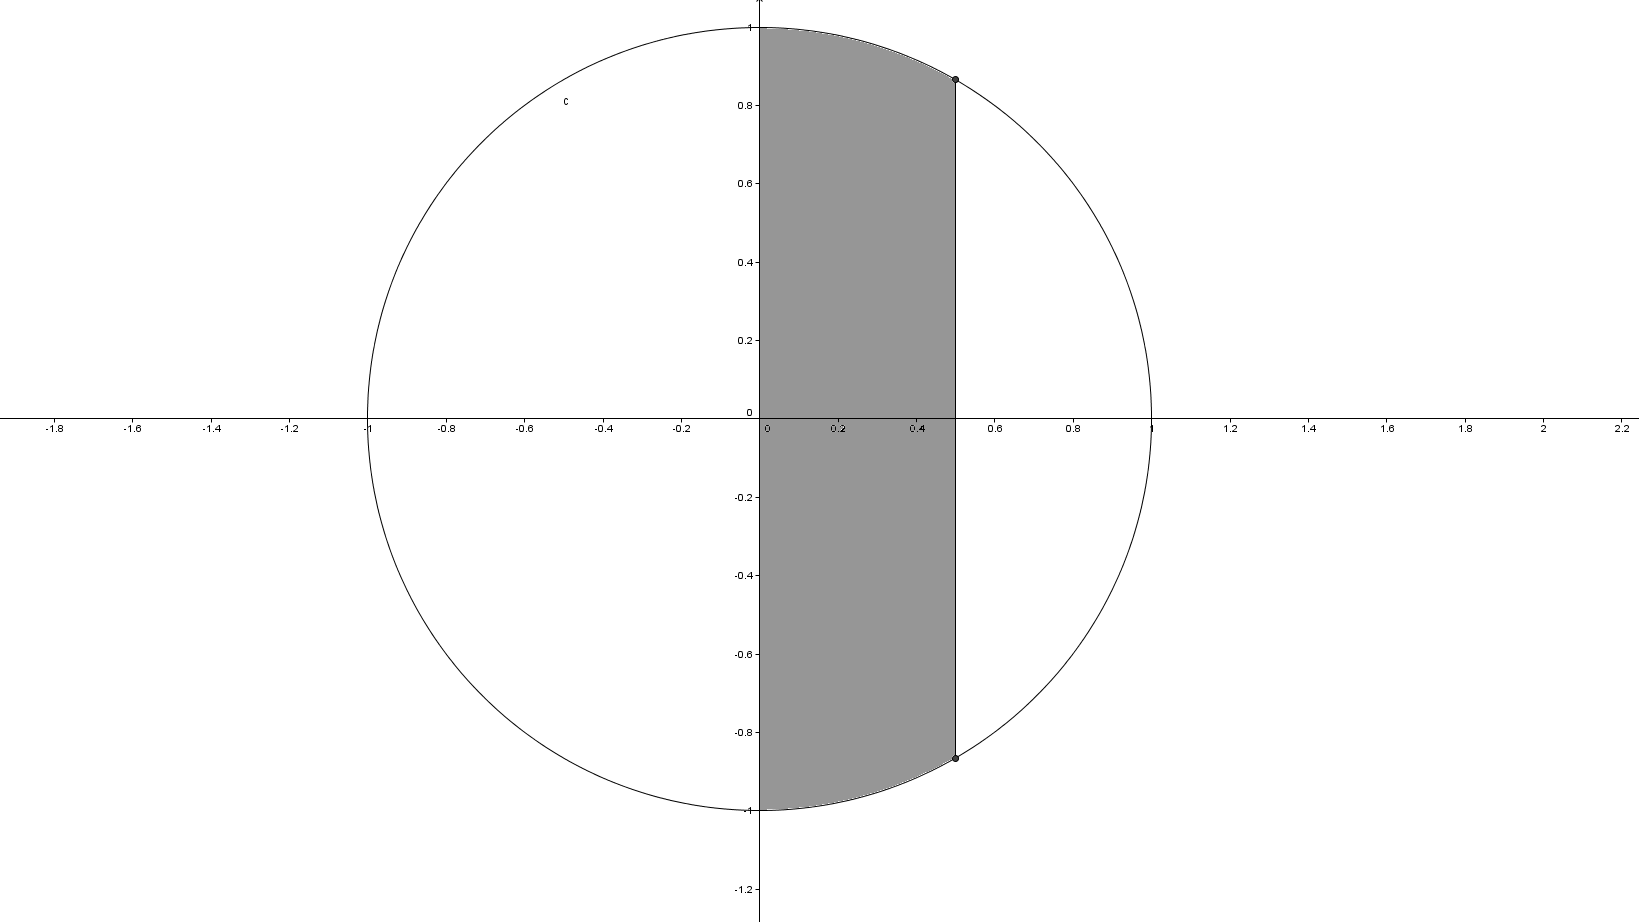
\includegraphics[height=7cm]{../fig/Cap04-Figura01-VariableAleatoriaContinua-bn.png}
	\end{bn}
	\caption{Cálculo de probabilidad en una variable aleatoria continua}
	\label{cap04:fig:EjemploVariableAleatoriaContinua}
    \end{figure}
el conjunto de puntos del círculo cuyas coordenadas $x$ están entre $0$ y $1/2$ tiene un área bien definida y no nula. ¿Cuánto vale ese área? Aproximadamente $0.48$, y esa es la probabilidad que buscábamos. El cálculo del área se puede hacer de distintas maneras, pero el lector debe darse cuenta de que en ejemplos como este se necesita a veces recurrir al cálculo de integrales.\\
    Naturalmente, se pueden hacer preguntas más complicadas. Por ejemplo, dado un punto $(x,y)$ del círculo $C$ podemos calcular el valor de $f(x,y)=x^2+ 4y^2$. Y entonces nos preguntamos ¿cuál es la probabilidad de que, tomando un punto al azar en $C$, el valor de $f$ esté entre 0 y 1? La respuesta es, de nuevo, un área, pero más complicada: es el área que se muestra en la Figura \ref{cap04:fig:EjemploVariableAleatoriaContinua2}.
    \begin{figure}[h]
	\centering
	\begin{enColor}
    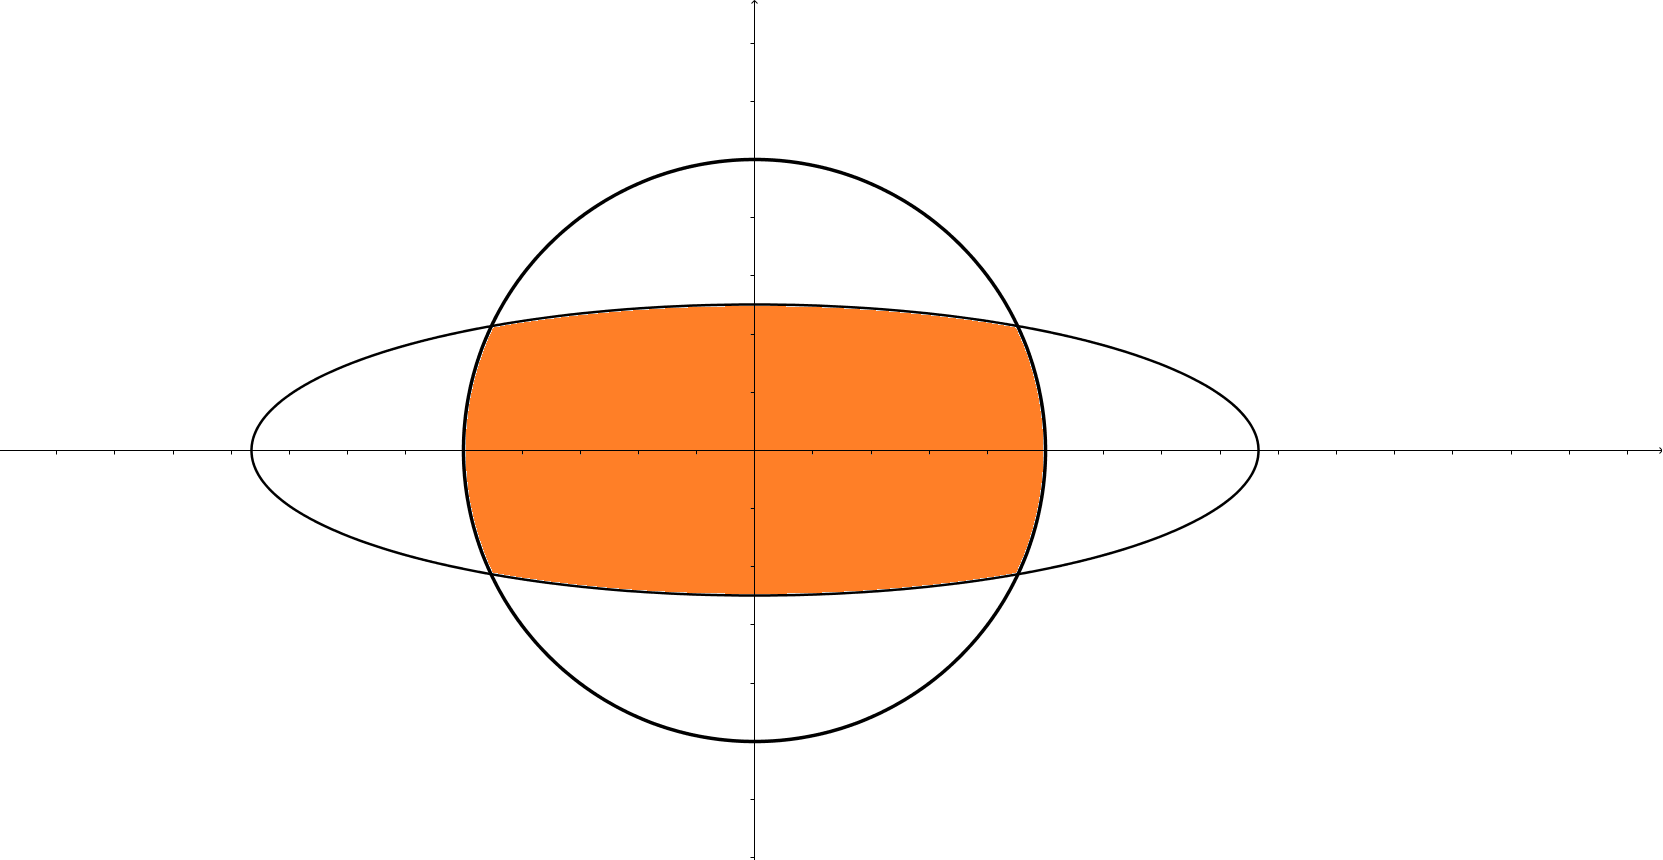
\includegraphics[height=7cm]{../fig/Cap04-Figura02-VariableAleatoriaContinua.png}
	\end{enColor}
	\begin{bn}
    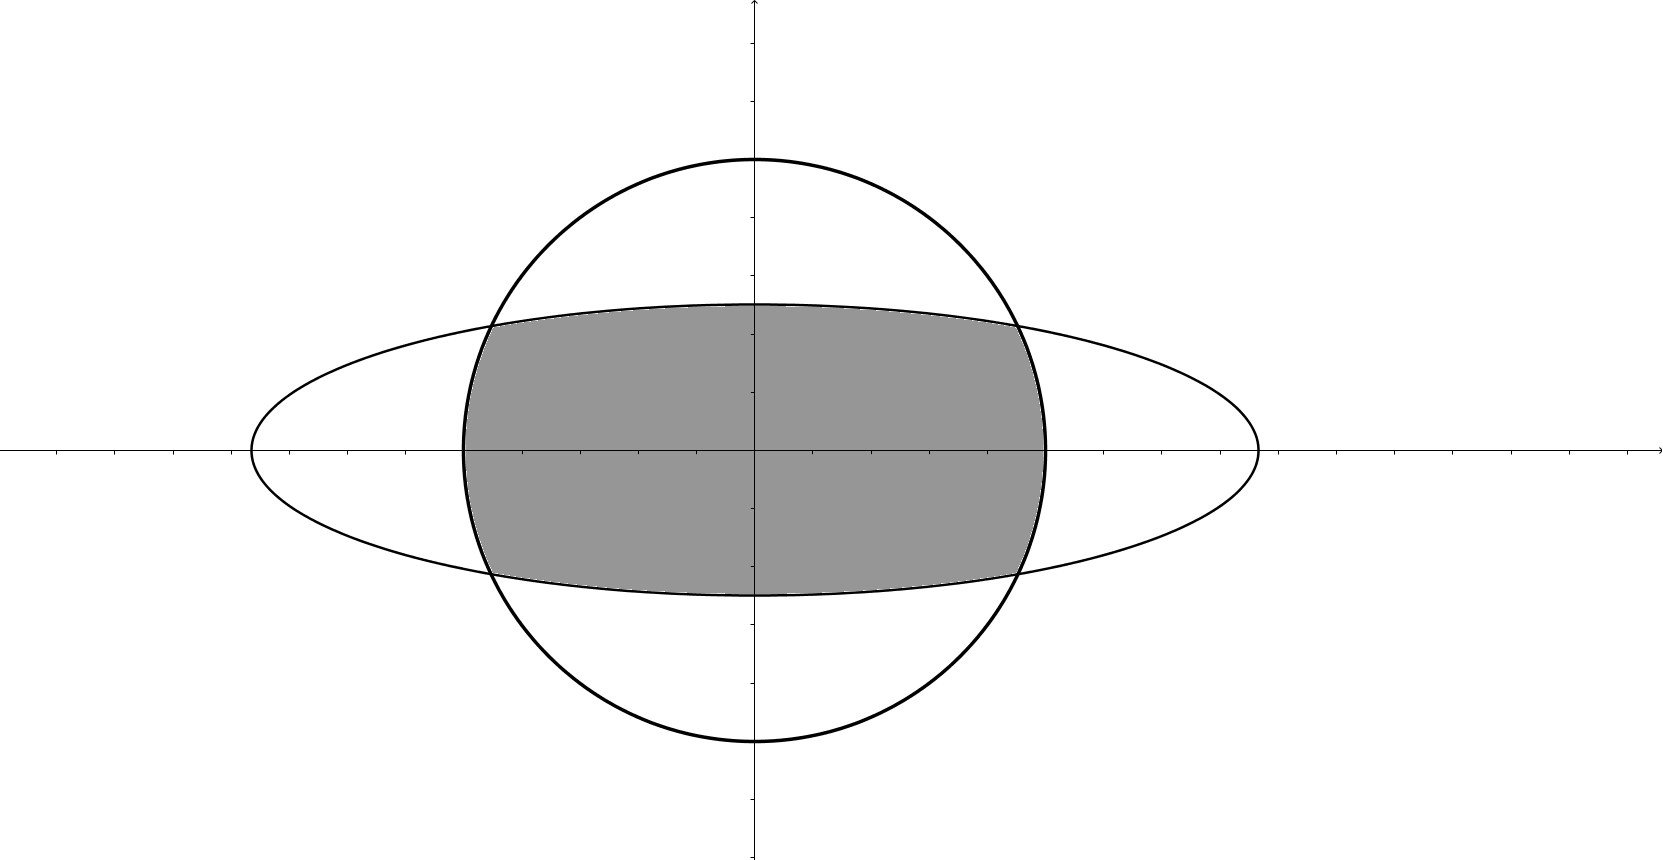
\includegraphics[height=7cm]{../fig/Cap04-Figura02-VariableAleatoriaContinua-bn.png}
	\end{bn}
	\caption{Un cálculo de probabilidad más complicado, para una variable aleatoria continua.}
	\label{cap04:fig:EjemploVariableAleatoriaContinua2}
    \end{figure}
    Lo que tienen en común ambos casos es que hay una función (o fórmula), que es $x$ en el primero y $f(x,y)$ en el segundo, y que nos preguntamos por la probabilidad de que los valores de esa fórmula caigan dentro de un cierto intervalo.
    \qed
\end{Ejemplo}
Los dos ejemplos que hemos visto contienen los ingredientes básicos de la noción de variable aleatoria. En el primer caso teníamos un conjunto finito de valores posibles, y a cada uno le asignábamos una probabilidad. En el segundo caso teníamos un recorrido continuo de valores posibles, y podíamos asignar probabilidades a intervalos. Lo que vamos a ver a continuación no se puede considerar de ninguna manera una definición rigurosa de variable aleatoria, pero servirá a nuestros propósitos.
    \begin{center}
    \fcolorbox{black}{Gris025}{
    \begin{minipage}{12cm}
        \begin{center}\bf Variables aleatorias:\end{center}
        Una {\sf variable aleatoria}\index{variable aleatoria} $X$ es una función (o fórmula) que le asigna, a cada elemento $p$ del espacio muestral $\Omega$, un número real $X(p)$. Distinguimos dos tipos de variables aleatorias:
        \begin{enumerate}
            \item La {\sf variable aleatoria $X$ es discreta}\index{variable aleatoria discreta} si sólo toma una cantidad finita (o una sucesión) de valores numéricos $x_1,x_2,x_3,\ldots$, de manera que para cada uno de esos valores tenemos bien definida la probabilidad $p_i=P(X=x_i)$ de que $X$ tome el valor $x_i$.
            \item La {\sf variable aleatoria $X$ es continua}\index{variable aleatoria continua} si sus valores forman un conjunto continuo dentro de los números reales (como una unión finita de intervalos, acotados o no), de manera que si nos dan un intervalo $I=(a,b)$ (aquí puede ser $a=-\infty$ o $b=+\infty$), tenemos bien definida la probabilidad $P(X\in I)$ de que el valor de $X$ esté dentro de ese intervalo $I$.
        \end{enumerate}
    \end{minipage}}
    \end{center}
¿Por qué no es una definición rigurosa? La situación es similar a lo que ocurría al definir los sucesos aleatorios. Un suceso aleatorio $A$ es un subconjunto que tiene bien definida la probabilidad $P(A)$. Pero, como ya hemos dicho, hay conjuntos tan {\em raros} que no es fácil asignarles un valor de la probabilidad, igual que a veces cuesta asignar un valor del área a algunas figuras muy raras. De la misma forma hay funciones tan raras que no se pueden considerar variables aleatorias. Se necesitan definiciones más rigurosas, pero que aquí sólo complicarían la discusión. Veamos un ejemplo, muy parecido al Ejemplo \ref{cap04:ejem:VariableAleatoriaSumaDosDados} (pág. \pageref{cap04:ejem:VariableAleatoriaSumaDosDados}).
\begin{Ejemplo}\label{ejem:VariableAleatoria:RestaDosDados}
    En el Ejemplo \ref{cap04:ejem:VariableAleatoriaSumaDosDados}, cada punto del espacio muestral es un par de números $(a,b)$, obtenidos al lanzar los dos dados. Podemos entonces definir una variable aleatoria $X$, que a cada punto $(a,b)$ del espacio muestral, le asigna la suma de esos dos valores:
    \[X(a,b)=a+b.\]
    En este caso, los valores de la probabilidad asignados por esta variable $X$ son los de la Tabla \ref{cap04:tabla:probabilidadSumaDados}.


    Siguiendo con este mismo espacio muestral, del lanzamiento de dos dados, en lugar de la suma ahora nos fijamos en la diferencia absoluta de los valores obtenidos (el mayor menos el menor, y cero si son iguales). Si llamamos $(a,b)$ al resultado de lanzar los dados, donde $a$ y $b$ son números del 1 al 6, entonces estamos definiendo una variable aleatoria mediante la expresión
    \[Y(a,b)=|a-b|.\]
    Esta claro que la variable $Y$ toma solamente los valores $0,1,2,3,4,5$. ¿Cuál es la probabilidad de que al calcular $Y$ obtengamos $3$? El siguiente diagrama ayudará a entender la respuesta. Para cada punto del espacio muestral se muestra el valor de $Y$:
    \[
    \begin{array}{cccccc}
    Y(1,1)=0&Y(1,2)=1&Y(1,3)=2&Y(1,4)=3&Y(1,5)=4&Y(1,6)=5\\
    Y(2,1)=1&Y(2,2)=0&Y(2,3)=1&Y(2,4)=2&Y(2,5)=3&Y(2,6)=4\\
    Y(3,1)=2&Y(3,2)=1&Y(3,3)=0&Y(3,4)=1&Y(3,5)=2&Y(3,6)=3\\
    Y(4,1)=3&Y(4,2)=2&Y(4,3)=1&Y(4,4)=0&Y(4,5)=1&Y(4,6)=2\\
    Y(5,1)=4&Y(5,2)=3&Y(5,3)=2&Y(5,4)=1&Y(5,5)=0&Y(5,6)=1\\
    Y(6,1)=5&Y(6,2)=4&Y(6,3)=3&Y(6,4)=2&Y(6,5)=1&Y(6,6)=0
    \end{array}
    \]
    Y se observa que $P(Y=3)=6/36=1/6$. De hecho, podemos repetir lo mismo para cada uno de los posibles valores de la variable aleatoria $Y$. Se obtiene la tabla de densidad de probabilidad que aparece como Tabla \ref{cap04:tabla:VariableAleatoriaDiferencia2Dados}.
    %Y de nuevo, insistimos, esta tabla es lo que en este caso caracteriza a la variable aleatoria diferencia $Y$. Se puede decir, sin riesgo de confusión, que {\sf\em esta tabla es la variable aleatoria $Y$. De la misma forma, la Tabla \ref{cap04:tabla:probabilidadSumaDados} define a la variable suma $X$.}
    \begin{table}[ht]
    \begin{center}
    \begin{tabular}[t]{|c|c|c|c|c|c|c|}
    \hline
    \rule{0cm}{0.5cm}{\em Valor de $Y$ (diferencia):}&0&1&2&3&4&5\\
    \hline
    \rule{0cm}{0.7cm}{\em Probabilidad de ese valor:}&$\dfrac{6}{36}$&$\dfrac{10}{36}$&$\dfrac{8}{36}$&$\dfrac{6}{36}$&$\dfrac{4}{36}$&$\dfrac{2}{36}$\\
    &&&&&&\\
    \hline
    \end{tabular}
    \end{center}
    \caption{Variable aleatoria diferencia al lanzar dos dados}\label{cap04:tabla:VariableAleatoriaDiferencia2Dados}
    \end{table}
    \qed
\end{Ejemplo}


\subsection{Variables aleatorias y sucesos. Función de densidad.}
\label{cap04:subsec:VariablesAleatoriasSucesos}

Al principio la diferencia entre suceso aleatorio y variable aleatoria puede resultar un poco confusa. Vamos a recordar lo que es cada uno de estos conceptos:
\begin{enumerate}
    \item Un suceso es un {\em subconjunto}, mientras que una variable aleatoria es una {\em función}. Por ejemplo, al lanzar dos dados, un suceso puede ser ``los dos resultados son pares'', y en este enunciado no hay un valor numérico fácil de identificar. Lo que sí tenemos es una {\em probabilidad asociada a este suceso}.
    \item Por el contrario, al considerar la variable aleatoria $Y(a,b)=|a-b|$, definida en el espacio muestral de los 36 resultados posibles, al lanzar dos dados, el valor numérico está claramente definido: $|a-b|$. Pero la definición de la operación {``diferencia en valor absoluto de los dados''}, por si misma, no define ningún suceso.
\end{enumerate}
¿Cuál es entonces el origen de la confusión? Posiblemente, la parte más confusa es que {\sf\em las variables aleatorias definen sucesos cuando se les asigna un valor}. Por ejemplo, si escribimos $Y(a,b)=|a-b|=3$, estamos pensando en el suceso {\em ``la diferencia de los resultados de los dados es 3''}. Es decir, el suceso formado por
\[\{(1,4),(2,5),(3,6),(6,3,),(5,2),(4,1)\}.\]
Y hemos visto en el Ejemplo \ref{ejem:VariableAleatoria:RestaDosDados} que la probabilidad de ese suceso es
\[P(Y=3)=1/6.\]
¿Para qué sirven entonces las variables aleatorias? Simplificando podemos decir que son, entre otras cosas, un atajo para hacer más sencillo el trabajo con sucesos. Precisando un poco más, su utilidad es que representan {\sf modelos abstractos de asignación (o distribución) de probabilidad}. Es decir, la variable aleatoria nos permite concentrar nuestra atención en la forma en que la probabilidad se reparte o {\em distribuye} entre los posibles resultados numéricos de un experimento aleatorio, sin entrar en detalles sobre el espacio muestral y los sucesos subyacentes a esa asignación de probabilidad.  Vamos a ver un par de ejemplos que tal vez ayude a aclarar el sentido en el que estas variables aleatorias son resúmenes que eliminan detalles (y por tanto, a menudo, información).
\begin{Ejemplo}\label{cap04:ejem:VariablesAleatoriasEliminanInformacion}
    Ya hemos discutido que en el espacio muestral correspondiente al lanzamiento de dos dados, la variable aleatoria $Y(a,b)=|a-b|$ tiene la tabla de densidad de probabilidades que se muestra en la Tabla \ref{cap04:tabla:VariableAleatoriaDiferencia2Dados} (pág. \pageref{cap04:tabla:VariableAleatoriaDiferencia2Dados}).
    Por su parte, la Tabla \ref{cap04:tabla:probabilidadSumaDados} (pág. \pageref{cap04:tabla:probabilidadSumaDados}) muestra la asignación (o densidad) de probabilidad de la variable aleatoria suma $X(a,b)=a+b$.
    En el Ejemplo \ref{Cap03:probabilidadCondicionadaLanzamientoDosDados} (página \pageref{Cap03:probabilidadCondicionadaLanzamientoDosDados}) nos hicimos la pregunta `` ¿Cuál es la probabilidad de que la diferencia entre los valores de ambos dados (mayor-menor) sea menor que 4, sabiendo que la suma de los dados es 7?''  Está claro, con la notación que usamos ahora, que estamos preguntando cuál es la probabilidad (condicionada) del suceso
    \[P\Big((Y<4)|(X=7)\Big).\]
    ¿Podemos calcular este número usando sólo las tablas de probabilidad de $X$ e $Y$, sin utilizar más información sobre el espacio muestral subyacente? La respuesta es que no, que necesitamos algo más de información. Volveremos sobre esta discusión en la Sección \ref{cap04:sec:IndependenciaVariablesAleatoriasDiscretas} (pág. \pageref{cap04:sec:IndependenciaVariablesAleatoriasDiscretas}).
    \qed
\end{Ejemplo}
En el siguiente ejemplo vamos a definir una variable aleatoria, cuyo espacio muestral subyacente se define con una variable de tipo cualitativo, un factor. Los factores, como sabemos, son  esencialmente etiquetas, y por lo tanto son realmente arbitrarios.  De la misma forma, al definir una variable aleatoria en un espacio muestral de ese tipo, los valores que asignamos a la variable aleatoria son completamente arbitrarios.
\begin{Ejemplo}\label{cap04:ejem:VariablesAleatoriasConFactorSubyacente}
    La baraja española típicamene tiene 48 naipes, o cartas, de los cuales 12 son figuras (sota, caballo y rey). Vamos a definir una variable aleatoria $X$ de la siguiente forma:
    \[
       X(\mbox{naipe})=\begin{cases}\phantom{-}1&\mbox{si el naipe es una figura}\\
       -1&\mbox{si el naipe no es una figura}
       \end{cases}
    \]
    ¿Por qué $1$ y $-1$? Podríamos haber utilizado cualesquiera otros dos valores. Pero tal vez estamos jugando un juego en el que, al extraer una carta al azar, nos pagan un euro si es una figura, o debemos pagar un euro si no lo es. Entonces esos valores arbitrarios pasan a representar el resultado, en euros, de la jugada. Aunque, naturalmente, se trata de un juego con unas reglas tan arbitrarias como los valores que hemos fijado para $X$.

    En cualquier caso, una vez definida la variable, y considerando que las cartas se extraen totalmente al azar de la baraja, de forma que todas las posibles cartas son equiprobables (ahí está implícito el reparto o distribución de probabilidad, vía la Regla de Laplace), entonces la variable $X$ es una variable como otras que hemos visto, con dos valores, cuyas correspondientes probabilidades aparecen en la Tabla \ref{cap04:tabla:VariableAleatoriaFiguraBarajaEspagnola}.
    \begin{table}[ht]
    \begin{center}
    \begin{tabular}[t]{|c|c|c|}
    \hline
    \rule{0cm}{0.5cm}{\em Valor de $X$}&1&-1\\
    \hline
    \rule{0cm}{0.7cm}{\em Probabilidad de ese valor:}&$\dfrac{12}{48}$&$\dfrac{36}{48}$\\
    &&\\
    \hline
    \end{tabular}
    \end{center}
    \caption{Variable aleatoria diferencia al lanzar dos dados}\label{cap04:tabla:VariableAleatoriaFiguraBarajaEspagnola}
    \end{table}
\qed
\end{Ejemplo}



\subsubsection*{Función de densidad de una variable aleatoria discreta.}
\label{cap04:subsubsec:FuncionDensidadVarAleatoriaDiscreta}

En el caso de las variables aleatorias discretas, hemos visto que es muy importante conocer la tabla de probabilidades asignadas a cada uno de los posibles valores de la variable. Para una variable aleatoria discreta que sólo toma una cantidad finita de valores numéricos $x_1,x_2,x_3,\ldots,x_k$, con probabilidades $p_i=P(X=x_i)$, esa tabla es como la Tabla \ref{cap04:tabla:tablaDensidadProbabilidadGenericaVariableAleatoriaDiscreta}.
    \begin{table}[h!]
    \begin{center}
    \begin{tabular}[t]{|c|c|c|c|c|c|}
    \hline
    \rule{0cm}{0.5cm}{\em Valor:}&$x_1$&$x_2$&$x_3$&$\cdots$&$x_k$\\
    \hline
    \rule{0cm}{0.7cm}{\em Probabilidad:}&$p_1$&$p_2$&$p_3$&$\cdots$&$p_k$\\
    \hline
    \end{tabular}
    \end{center}
    \caption{Tabla de densidad de probabilidad de una variable aleatoria discreta (con un número finito de valores)}\label{cap04:tabla:tablaDensidadProbabilidadGenericaVariableAleatoriaDiscreta}
    \end{table}
Esta tabla se conoce como {\sf función de densidad de probabilidad, o función de masa}\index{función de masa}\index{función de densidad de probabilidad, variable aleatoria discreta} de la variable aleatoria $X$.

¿Por qué la llamamos función si es una tabla? Bueno, una posible respuesta es que para casos como estos (donde sólo hay una cantidad finita de valores posibles), en realidad una tabla es lo mismo que una función. Probablemente el lector tiene la idea de que una función es, de alguna manera, una {\em fórmula}. Para los matemáticos la idea es algo más general. Una función es un objeto que permite asignar un valor, ya sea mediante una fórmula, una tabla, o siguiendo un conjunto de instrucciones como en un programa de ordenador. Así que no hay problema en decir que la Tabla \ref{cap04:tabla:tablaDensidadProbabilidadGenericaVariableAleatoriaDiscreta} es una función de densidad.

Quizá se empiece a entender un poco más la terminología al pensar en situaciones como las del Ejemplo \ref{Cap03:ejem:LanzamientoMonedaHastPrimeraCara}, (página \pageref{Cap03:ejem:LanzamientoMonedaHastPrimeraCara}), aquel  en el que lanzábamos monedas hasta obtener la primera cara. Supongamos que en ese ejemplo definimos la variable aleatoria
\[X=\mbox{número de lanzamientos hasta la primera cara.}\]
¿Cómo sería la ``tabla'' de densidad de probabilidad correspondiente a ese ejemplo? Usando los resultados del Ejemplo \ref{cap03:ejem:LanzamientoMonedaHastPrimeraCara:2} (pág. \pageref{cap03:ejem:LanzamientoMonedaHastPrimeraCara:2}), podemos ver que sería una especie de tabla infinita como la Tabla \ref{cap04:tabla:tablaDensidadProbabilidadInfinita}.
    \begin{table}[h!]
    \begin{center}
    \begin{tabular}[t]{|c|c|c|c|c|c|c}
    \hline
    \rule{0cm}{0.5cm}{\em Valor:}&$1$&$2$&$3$&$\cdots$&$k$&$\cdots$\\
    \hline
    \rule{0cm}{0.7cm}{\em Probabilidad:}&$\dfrac{1}{2}$&$\dfrac{1}{2^2}$&$\dfrac{1}{2^3}$&$\cdots$&$\dfrac{1}{2^k}$&$\cdots$\\[4mm]
    \hline
    \end{tabular}
    \end{center}
    \caption{``Tabla infinita'' de densidad de probabilidad para la variable aleatoria del Ejemplo \ref{Cap03:ejem:LanzamientoMonedaHastPrimeraCara}}\label{cap04:tabla:tablaDensidadProbabilidadInfinita}
    \end{table}
En una situación como esta, donde vemos que la variable $X$ toma los valores $1,2,3,\ldots,k,\ldots$, es mucho más cómodo utilizar notación funcional y decir que la función de densidad de $X$ es:
\[f(X=k)=P(X=k)=\dfrac{1}{2^k}.\]
Esto se traduce en esta definición, más formal:
    \begin{center}
    \fcolorbox{black}{Gris025}{
    \begin{minipage}{12cm}
    %\begin{definicion}
        {\bf Función de densidad de una variable aleatoria discreta}\\
        \index{función de densidad de una variable aleatoria discreta}
        Si $X$ es una variable aleatoria discreta, su {\sf función de densidad (de probabilidad)} es la función definida mediante:
        \begin{equation}
        \label{cap04:ecu:funcionDensidadVariableAleatoriaDiscreta}
            f(x)=P(X=x),\mbox{ para cualquier número real }x.
        \end{equation}
    %\end{definicion}
    \end{minipage}}
    \end{center}
Por supuesto, la función de densidad vale 0 en aquellos valores que $X$ no toma. La notación es importante: se suele emplear una letra $f$ minúscula para representar a la función de densidad. Cuando sea necesario, especialmente para evitar confusiones al trabajar con varias variables aleatorias, usaremos la notación $f_X$ para indicar que nos referimos a la función de densidad de la variable aleatoria $X$.

Aunque la llamemos función de densidad, vamos a seguir pensando muchas veces en ella como una tabla, porque eso a menudo ayuda a nuestra intuición. En particular, conviene tener presente que, puesto que las probabilidades se pueden pensar (de nuevo, intuitivamente) como la versión teórica de las frecuencias relativas, una tabla de probabilidades es una imagen teórica de las tablas de frecuencias relativas que veíamos en el Capítulo \ref{cap:ValoresCentralesDispersion}. Nos estamos refiriendo a frecuencias relativas, pero en el Capítulo \ref{cap:ValoresCentralesDispersion} vimos que también podíamos considerar las {\em frecuencias relativas acumuladas}, y que eran útiles para entender algunas características de los datos. ¿Cuál sería el análogo teórico de las frecuencias relativas acumuladas? ¿Algo así como las {\em ``probabilidades acumuladas''?} En efecto, eso es exactamente lo que vamos a hacer más adelante en este capítulo, en la Sección \ref{cap04:sec:FuncionDistribucionVariableAleatoriaDiscreta}, aunque le daremos otro nombre al resultado de nuestro trabajo.

En el caso de las variables aleatorias continuas, no podemos hacer la asignación de probabilidades de esta misma forma. Recordando que la probabilidad de las variables continuas es análoga al área, necesitamos un recurso técnicamente más complicado: el cálculo de áreas, en Matemáticas, recurre al cálculo de integrales. {!`}No hay que asustarse! Trataremos ese problema más adelante, pero ya  adelantamos que vamos a esforzarnos para que esos detalles técnicos no nos impidan ver las ideas que se esconden detrás.


\section{Media y varianza de variables aleatorias.}\label{cap04:sec:MediaVarianzaVariablesAleatorias}


\subsection{Media de una variable aleatoria discreta.}
\label{cap04:subsec:MediaVariableAleatroriaDiscreta}

Hemos visto que las variables aleatorias son modelos teóricos de asignación de probabilidad, entre los resultados distintos de un experimento aleatorio. Y de la misma forma que hemos aprendido a describir un conjunto de datos mediante su media aritmética y su desviación típica, podemos
describir a una variable aleatoria mediante valores similares. Empecemos por la media, en el caso de una variable aleatoria discreta. El caso de las variables aleatorias continuas requiere, como hemos dicho, la ayuda del Cálculo Integral, y lo veremos un poco más adelante.

El punto de partida es la fórmula que ya conocemos para calcular la media aritmética de una variable discreta a partir de su tabla de frecuencias, que escribimos de una forma ligeramente diferente, usando las frecuencias relativas:
    \[
    \bar x=\dfrac{\displaystyle\sum_{i=1}^k x_i\cdot f_i}{\displaystyle\sum_{i=1}^k f_i}
    =\dfrac{\displaystyle\sum_{i=1}^k x_i\cdot f_i}{n}
    =\displaystyle\sum_{i=1}^k x_i\cdot \dfrac{f_i}{n}
    \]
y aquí $\dfrac{f_i}{n}$ es la frecuencia relativa número $i$.\\[3mm]
Para entender el siguiente paso, es importante tener presente que la probabilidad, como concepto teórico, es una idealización de lo que sucede en la realidad que estamos tratando de representar. Para centrar las ideas, volvamos al conocido caso del lanzamiento de dos dados, que ya hemos visto en el Ejemplo \ref{ejem:VariableAleatoria:RestaDosDados} (página \pageref{ejem:VariableAleatoria:RestaDosDados}).
\begin{Ejemplo}
[\bf Continuación del Ejemplo \ref{ejem:VariableAleatoria:RestaDosDados}]
\label{ejem:Cap04-VariableAleatoria:SumaDosDados}
    De nuevo, pensamos en la variable aleatoria $X$, suma de los resultados al lanzar dos dados.
    La Tabla \ref{cap04:tabla:probabilidadSumaDados} (pág. \pageref{cap04:tabla:probabilidadSumaDados}) muestra la asignación o densidad de probabilidades para los posibles valores de la suma. Pero esto es un modelo teórico que describe a la variable aleatoria suma. Si hacemos un experimento en el mundo real, como el lanzamiento de 3000 pares de dados, lo que obtendremos es una tabla de {\em frecuencias relativas} que son {\em aproximadamente} iguales a las probabilidades. ¿Y si en lugar de lanzar 3000 veces lo hiciéramos un millón de veces? En el Tutorial04 tendrás ocasión de usar el ordenador para responder a esta pregunta.
    \qed
\end{Ejemplo}
La idea que queremos subrayar es que, en el caso de los dados, los valores de las probabilidades son una especie de límite teórico de las frecuencias relativas, una idealización de lo que ocurre si lanzamos los dados muchísimas veces, tendiendo hacia infinito. Y por lo tanto, esto parece indicar que, cuando pasamos de la realidad (donde viven las frecuencias observadas) al modelo teórico (en el que viven las probabilidades ideales), las fórmulas teóricas correctas se obtienen cambiando las frecuencias relativas por las correspondientes probabilidades. Eso conduce a esta definición para la media de una variable aleatoria:
    \begin{center}
    \fcolorbox{black}{Gris025}{
    \begin{minipage}{12cm}
        \begin{center}
        \bf Media $\mu$ de una variable aleatoria discreta (valor esperado o esperanza)
        \index{valor esperado de una variable aleatoria discreta}
        \index{esperanza de una variable aleatoria discreta}
        \index{media de una variable aleatoria discreta}
        \end{center}
        Si $X$ es una variable aleatoria discreta, que toma los valores $x_1,x_2,\ldots,x_k$, con las probabilidades $p_1,p_2,\ldots,p_k$ (donde $p_i=P(X=x_i)$), entonces la {\sf media}, o {\sf valor esperado}, o {\sf esperanza matemática}  de $X$ es:
        \begin{equation}\label{cap04:ecu:MediaVariableDiscreta}
        \mu=\sum_{i=1}^k
        \left(x_i\cdot P(X=x_i)\right)=x_1p_1+x_2p_2+\cdots+x_kp_k.
        \end{equation}
    \end{minipage}
    }
    \end{center}
La media de una variable aleatoria discreta se suele representar con la letra griega $\mu$ para distinguirla de la media aritmética de unos datos $\bar x$, que hemos visto en capítulos previos. La media de una variable aleatoria, como hemos indicado, también se suele llamar valor esperado o esperanza matemática de la variable $X$.

Cuando trabajemos con varias variables, y haya riesgo de confusión, usaremos una notación de subíndices, como $\mu_X$, para indicar la variable aleatoria a la que corresponde esa media.

Una observación más sobre esta definición: en el caso de que la variable aleatoria tome infinitos valores (ver el Ejemplo \ref{Cap03:ejem:LanzamientoMonedaHastPrimeraCara}, página \pageref{Cap03:ejem:LanzamientoMonedaHastPrimeraCara}), en el que lanzábamos monedas hasta obtener la primera cara, esta suma puede ser una suma con infinitos sumandos; lo que en Matemáticas se llama una {\sf serie}.

Vamos a aplicar esta definición al ejemplo de la suma de dos dados
    \begin{Ejemplo}
    \label{ejem:Cap04:VariableAleatoriaSumaDosDadosMedia}
    {\bf Continuación del Ejemplo \ref{ejem:Cap04-VariableAleatoria:SumaDosDados}}\\
    Seguimos trabajando con la variable aleatoria $X$, suma de los resultados al lanzar dos dados.
    Su tabla de densidad de probabilidad es la Tabla \ref{cap04:tabla:probabilidadSumaDados} (pág. \pageref{cap04:tabla:probabilidadSumaDados}), que reproducimos aquí por comodidad:
    \begin{center}
    {\small
    \begin{tabular}[t]{|c|c|c|c|c|c|c|c|c|c|c|c|}
    \hline
    Valor\rule{0cm}{0.5cm}
    &2&3&4&5&6&7&8&9&10&11&12\\
    \hline
    Probabilidad\rule{0cm}{0.7cm}
    &$\dfrac{1}{36}$&$\dfrac{2}{36}$&$\dfrac{3}{36}$&$\dfrac{4}{36}$&$\dfrac{5}{36}$&$\dfrac{6}{36}$&$\dfrac{5}{36}$&$\dfrac{4}{36}$&$\dfrac{3}{36}$&$\dfrac{2}{36}$&$\dfrac{1}{36}$\\
    &&&&&&&&&&&\\
    \hline
    \end{tabular}
    }
    \end{center}
    A partir de la tabla tenemos:
    \[\mu=\sum x_i P(X=x_i)=\mbox{\small $
    2\cdot\dfrac{1}{36}+3\cdot\dfrac{2}{36}+4\cdot\dfrac{3}{36}+5\cdot\dfrac{4}{36}+6\cdot\dfrac{5}{36}+$}\]
    \[\mbox{\small $
    7\cdot\dfrac{6}{36}+8\cdot\dfrac{5}{36}+9\cdot\dfrac{4}{36}+10\cdot\dfrac{3}{36}+11\cdot\dfrac{2}{36}
    +12\cdot\dfrac{1}{36}$}=7.\]
    Así que, en este ejemplo, la media o valor esperado es $\mu=7$.

    Dejamos como ejercicio para el lector, comprobar que la media de la variable diferencia $Y(a,b)=|a-b|$ del Ejemplo \ref{ejem:VariableAleatoria:RestaDosDados} (pág. \pageref{ejem:VariableAleatoria:RestaDosDados}) es:
    \[\mu_Y=\dfrac{35}{18}\approx 1.944\]
    \qed
    \end{Ejemplo}

\subsubsection*{Valor esperado y juegos justos.}

Cuando se usa la probabilidad para analizar un juego de azar en el que cada jugador invierte una cierta cantidad de recursos (por ejemplo, dinero), es conveniente considerar la variable aleatoria
    \[X=\mbox{beneficio del jugador}=\mbox{(ganancia neta)}-\mbox{(recursos invertidos)}.\]
Para que el juego sea justo\index{juego justo}\index{justo, juego} la media de la variable beneficio (es decir, el beneficio esperado) debería ser $0$. Veamos un ejemplo.
\begin{ejemplo}\label{cap04:ejem:JuegosJustos}
Tenemos una caja con $7$ bolas blancas y 4 bolas negras. El juego consiste en lo siguiente. Tu pones un euro, y yo pongo $x$ euros. Sacamos una bola de la caja al azar. Si es negra, ganas tú y te quedas con todo el dinero (tu apuesta y la mía). Si la bola es blanca, gano yo y me quedo todo el dinero. ¿Cuántos euros debo poner yo para que el juego sea justo?

Lo que debemos hacer es, simplemente, calcular el valor medio o valor esperado de la variable aleatoria:
\[X=\mbox{(tu beneficio)}.\]
Esta variable toma dos valores. Se tiene $X=-1$ cuando la bola es blanca, y pierdes el euro que has apostado. Y se tiene $X=x$ si la bola es negra y tú ganas todo el dinero (tu euro, y mis $x$ euros; en este caso tu beneficio es $x$ porque hay que descontar el euro que has invertido). La tabla de densidad de probabilidad para $X$ es esta:
\begin{center}
    \begin{tabular}[t]{|c|c|c|}
    \hline
    Valor de $X$:\rule{0cm}{0.5cm}
    &$x$&$-1$\\
    \hline
    Probabilidad:\rule{0cm}{0.7cm}
    &$\,\,\dfrac{4}{11}$&$\dfrac{7}{11}$\\[2mm]
    &\mbox{(bola negra)}&\mbox{(bola blanca)}\\
    \hline
    \end{tabular}
\end{center}
así que el valor esperado es:
\[\mu_X=x\cdot\dfrac{4}{11}+(-1)\cdot\dfrac{7}{11}=\dfrac{4x-7}{11}.\]
Para que el juego sea justo, el valor medio $\mu_X$ debe ser $0$. Despejando, se obtiene que mi apuesta debe ser de $x=\frac{7}{4}$ de euro, es decir un euro y $75$ céntimos.  Dejamos como ejercicio para el lector comprobar que se obtiene el mismo resultado si, en lugar de la variable $X=$(tu beneficio), se usa la variable $Y=$(mi beneficio).
\qed
\end{ejemplo}
%El siguiente ejemplo
%
%
%
%
%
%\begin{Ejemplo}
%    Cada uno de nosotros pone un euro, y lanzamos un dado. Si sale un uno ganas tú y te quedas los dos euros. Si sale cualquier otra cosa gano yo y me quedo los dos euros. ¿Es un juego justo? Parece claro que no. ¿Cuál es el valor esperado del beneficio para cada uno de nosotros?\\
%    Una pregunta más interesante. Si tú sigues poniendo un euro, ¿cuántos euros tengo que poner yo para que el juego sea justo?\qed
%\end{Ejemplo}
Por cierto, esencialmente ninguna de las loterías, sorteos o juegos de azar legales es justa en este sentido (de los ilegales, ni hablemos). Cada uno es libre de creer en su suerte, pero nunca deberíamos confundirla con la esperanza... y menos, con la esperanza matemática.

Esta definición de juego justo está muy relacionada con las reglas de las apuestas que discutimos en la Sección (opcional) \ref{cap03:sec:OddsPruebasDiagnosticas} (pág. \pageref{cap03:sec:OddsPruebasDiagnosticas}). Vamos a verlo en un ejemplo, pero por supuesto, con la advertencia de que si aún no has leído esa sección, debes ignorar este ejemplo y el que le sigue.
\begin{ejemplo}\label{cap04:ejem:OddsReglasApuestasJuegoJusto}
{\bf (Continuación del Ejemplo \ref{cap03:ejem:OddsReglasApuestas}, ver pág. \pageref{cap03:ejem:OddsReglasApuestas})}
Las cuentas que hemos hecho en el Ejemplo \ref{cap03:ejem:OddsReglasApuestas} consisten esencialmente en demostrar que las reglas de las apuestas definen un juego justo para el corredor de apuestas (su beneficio esperado era $0$ euros). Vamos a hacer ahora las cuentas para un jugador que apuesta a favor de $A$. Recordemos que en aquel ejemplo, las posibilidades (odds) en contra de $A$ eran de $1$ a $7$. Es decir,
\[O_A=\dfrac{1}{7}.\]
Por lo tanto,
\[P(A)=\dfrac{1}{8},\quad  P(A^c)=\dfrac{7}{8}.\]
Y teniendo en cuenta que el jugador invierte un euro, y si gana obtiene $8$ euros, su beneficio esperado es:
\[(-1)\cdot\dfrac{1}{8}+8\cdot\dfrac{7}{8}=0.\]
Así que el juego también es justo para los apostadores (dejamos como ejercicio comprobar que lo es para quienes apuestan por $A^c$).
\qed
\end{ejemplo}
Para ver como la noción de posibilidades (odds) puede simplificar el análisis de un juego de apuestas, volvamos sobre el primer ejemplo que hemos discutido.
\begin{ejemplo}
\label{cap04:ejem:JuegosJustos01}
{\bf (Continuación del Ejemplo \ref{cap04:ejem:JuegosJustos})}
Puesto que la caja tiene $4$ bolas negras y siete blancas, las posibilidades (odds) a favor de bola negra son
\[O_{negra}=\dfrac{4}{7}.\]
Y para que el juego sea justo, el cociente entre lo que apuestas tú y lo que apuesto yo, debe ser igual a esas posibilidades:
\[\dfrac{1}{x}=\dfrac{4}{7}.\]
El resultado, de nuevo, es $x=7/4$.
\qed
\end{ejemplo}



\subsection{Varianza y desviación típica de una variable aleatoria discreta.}
\label{cap04:subsec:VarianzaDesvTipicaVariableAleatoriaDiscreta}

Ahora que hemos visto la definición de media, y cómo obtenerla a partir de la noción de frecuencias relativas, parece bastante evidente lo que tenemos que hacer para definir la varianza de una variable aleatoria discreta. Recordemos la fórmula para la varianza poblacional a partir de una tabla de frecuencias, y vamos a escribirla en términos de frecuencias relativas:
    \[
    \mbox{Var($x$)}=\dfrac{\displaystyle\sum_{i=1}^k{ f_i\cdot}(x_i-\bar x)^2}{{ \displaystyle\sum_{i=1}^k f_i}}=
    \dfrac{\displaystyle\sum_{i=1}^k{ f_i\cdot}(x_i-\bar x)^2}{n}=
    \displaystyle\sum_{i=1}^k{(x_i-\bar x)^2\cdot}\dfrac{f_i}{n}.
   \]
Por lo tanto, definimos:
%
%
%   \begin{center}%\\[3mm]
%   \fbox{\colorbox{Gris025}{\begin{minipage}{14cm}
%   \begin{center}
%   \vspace{2mm}
%   {\bf Varianza $\sigma^2$ de una variables aleatoria discreta: }
%   \index{Varianza de una variables aleatoria discreta}
%   \end{center}
%   La {\sf varianza}  de una variable aleatoria discreta $X$, que toma los valores $x_1,x_2,x_3,\ldots,x_k$, con las probabilidades $p_1,p_2,\ldots,p_k$ (donde $p_i=P(X=x_i)$), es:
%   \[
%   \sigma^2=\sum_{i=1}^k
%   \left((x_i-\mu)^2P(X=x_i)\right).
%   \]
%   \end{minipage}}}\end{center}%\\[3mm]
    \begin{center}
    \fcolorbox{black}{Gris025}{
    \begin{minipage}{12cm}
        \begin{center}
        \bf Varianza $\sigma^2$ de una variable aleatoria discreta
        \index{varianza de una variable aleatoria discreta}
        \end{center}
       La {\sf varianza}  de una variable aleatoria discreta $X$, que toma los valores $x_1,x_2,x_3,\ldots,x_k$, con las probabilidades $p_1,p_2,\ldots,p_k$ (donde $p_i=P(X=x_i)$), es:
       \[
       \sigma^2=\sum_{i=1}^k
       \bigg((x_i-\mu)^2\cdot P(X=x_i)\bigg).
       \]
    \end{minipage}
    }
    \end{center}
Y por supuesto, esta definición va acompañada por la de la desviación típica:
    \begin{center}
    \fcolorbox{black}{Gris025}{
    \begin{minipage}{12cm}
        \begin{center}
        \bf Desviación típica $\sigma$ de una variable aleatoria discreta
        \index{desviación típica de una variables aleatoria discreta}
        \end{center}
       La {\sf desviación típica}  de una variable aleatoria discreta $X$ es simplemente la raíz cuadrada $\sigma$ de su varianza.
           \[
           \sigma=\displaystyle\sqrt{\sum_{i=1}^k\left((x_i-\mu)^2P(X=x_i)\right)}.
           \]
    \end{minipage}
    }
    \end{center}
Para ilustrar las definiciones anteriores, vamos a calcular la varianza y desviación típica de la variable aleatoria
\begin{Ejemplo}[\bf Continuación del Ejemplo \ref{ejem:Cap04:VariableAleatoriaSumaDosDadosMedia}, pág. \pageref{ejem:Cap04:VariableAleatoriaSumaDosDadosMedia}]
\label{cap04:ejem:varianzaVariableAleatoriaDiscreta}
Para la variable aleatoria $X$, suma de los resultados al lanzar dos dados, hemos obtenido $\mu=7$. Ahora, usando su tabla de densidad de probabilidades, tenemos
    \[\sigma^2=\sum (x_i-\mu)^2 P(X=x_i)=\]
    \[\mbox{\small $
    (2-7)^2\cdot\dfrac{1}{36}+(3-7)^2\cdot\dfrac{2}{36}+(4-7)^2\cdot\dfrac{3}{36}+(5-7)^2\cdot\dfrac{4}{36}+(6-7)^2\cdot\dfrac{5}{36}+(7-7)^2\cdot\dfrac{6}{36}$}\]
    \[\mbox{\small $
    +(8-7)^2\cdot\dfrac{5}{36}+(9-7)^2\cdot\dfrac{4}{36}+(10-7)^2\cdot\dfrac{3}{36}+(11-7)^2\cdot\dfrac{2}{36}
    +(12-7)^2\cdot\dfrac{1}{36}$}=\dfrac{35}{6}\approx 5.833\]
Así que la varianza de $X$ es $\sigma^2=\dfrac{35}{6}$, y su desviación típica, obviamente, es \[\sigma=\sqrt{\dfrac{35}{6}}\approx 2.415\]
Dejamos como ejercicio para el lector, comprobar que la varianza de la variable diferencia $Y(a,b)=|a-b|$ del Ejemplo \ref{ejem:VariableAleatoria:RestaDosDados} (pág. \pageref{ejem:VariableAleatoria:RestaDosDados}) es:
\[\sigma^2_Y=\dfrac{665}{324}\approx 2.053\]
\qed
\end{Ejemplo}

\section{Operaciones con variables aleatorias.}
\label{sec:OperacionesVariablesAleatorias}

Para facilitar el trabajo, aparte de los símbolos $\mu$ y $\sigma^2$ que ya vimos, para la media y varianza de una variable aleatoria, en esta sección vamos a usar otros símbolos para esas mismas cantidades. En concreto, vamos a usar:
    \[E(X)=\mu,\qquad \qquad \operatorname{Var}(X)=\sigma^2,\]
para la media y la varianza respectivamente. Estos símbolos son a veces más cómodos cuando se trabaja a la vez con varias variables aleatorias, o se hacen {\em operaciones} con las variables aleatorias.

¿Qué queremos decir con esto? Una variable aleatoria $X$ es, al fin y al cabo, una fórmula que produce un resultado numérico. Y puesto que es un número, podemos hacer operaciones con ella. Por ejemplo, tiene sentido hablar de $2X$, $X+1$, $X^2$, etcétera.
\begin{Ejemplo}
\label{cap04:ejem:OperacionesVariablesAleatorias01}
    En el caso del lanzamiento de dos dados, teníamos la variable aleatoria suma, definida mediante $X(a,b)=a+b$. En este caso:
    \[
    \begin{cases}
    2X(a,b)=2a+2b\\[2mm]
    X(a,b)+1=a+b+1\\[2mm]
    X^2(a,b)=(a+b)^2
    \end{cases}
    \]
    de manera que, por ejemplo, $X^2(3,4)=(3+4)^2=49$.\qed
\end{Ejemplo}

De la misma manera, si tenemos dos variables aleatorias $X_1$ y $X_2$ (dos fórmulas), definidas sobre el mismo espacio muestral, podemos sumarlas para obtener una nueva variable $X=X_1+X_2$. También, por supuesto, podemos multiplicarlas, dividirlas, etcétera.
\begin{Ejemplo}
    De nuevo en el lanzamiento de dos dados, si consideramos la variable aleatoria suma $X_1(a,b)=a+b$, y la variable aleatoria producto $X_2(a,b)=a\cdot b$, sería:
    \[X_1(a,b)+X_2(a,b)=(a+b)+a\cdot b.\]
    \qed
\end{Ejemplo}
Si hemos invertido algo de tiempo y esfuerzo en calcular las medias y las varianzas $X_1$ y $X_2$, nos gustaría poder aprovechar ese esfuerzo para obtener sin complicaciones las medias y varianzas de combinaciones sencillas, como $X_1+X_2$, o $3X_1+5$, etcétera. Afortunadamente, eso es posible en el caso de la media. Para la varianza, sin embargo, en el caso de dos variables, vamos a tener que  imponer un requisito técnico adicional.
    \begin{center}
    \fcolorbox{black}{Gris025}{
    \begin{minipage}{12cm}
        \begin{center}
        \bf Media y varianza de una combinación lineal de variables aleatorias
        \label{cap04:lugar:OperacionesVariablesAleatorias}
        \index{media de una combinación lineal de variables aleatorias}
        \index{varianza de una combinación lineal de variables aleatorias}
        \end{center}
           \begin{itemize}
           \item Si $X$ es una variable aleatoria, y $a, b$ son números cualesquiera, entonces
           \[E(a\cdot X+b)=a\cdot E(X)+b,\quad \operatorname{Var}(a\cdot X+b)=a^2\cdot \operatorname{Var}(X).\]
           \item Y si $X_1, X_2$ son dos variables aleatorias, se tiene:
           \[E(X_1+X_2)=E(X_1)+E(X_2).\]
           Si además $X_1$ y $X_2$ son {\sf\em independientes}, entonces
           \[\operatorname{Var}(X_1+X_2)=\operatorname{Var}(X_1)+\operatorname{Var}(X_2).\]
           \end{itemize}
    \end{minipage}
    }
    \end{center}
No entramos en este momento en la definición técnica de la independencia, pero es fácil intuir que se basa en la independencia de los sucesos subyacentes a los valores de las variables. En la Sección \ref{cap04:sec:IndependenciaVariablesAleatoriasDiscretas} daremos una definición rigurosa.

Con la notación de $\mu$ y $\sigma$ se obtienen estas fórmulas, algo menos legibles:
    \[\mu_{aX+b}=a\cdot\mu_X + b,\quad \sigma^2_{aX+b}=a^2\sigma^2_X\]
y
\[\mu_{X_1+X_2}=\mu_{X_1}+\mu_{X_2},\quad \sigma^2_{X_1+X_2}=\sigma^2_{X_1}+\sigma^2_{X_2},\]
donde la última fórmula, insistimos, {\em es válida para variables independientes}.

Veamos un ejemplo:
\begin{Ejemplo}
\label{cap04:ejem:varianzaSumaVariablesAleatoriasDiscretas}
Consideramos las variables aleatorias $X$ (suma) e $Y$ (diferencia), del ejemplo \ref{ejem:VariableAleatoria:RestaDosDados} (pág. \pageref{ejem:VariableAleatoria:RestaDosDados}). Vamos a calcular $\operatorname{Var}(X+Y)$. En el Ejemplo \ref{cap04:ejem:varianzaVariableAleatoriaDiscreta} (pág. \pageref{cap04:ejem:varianzaVariableAleatoriaDiscreta}) hemos visto que \[\operatorname{Var}(X)=\dfrac{35}{6},\qquad \operatorname{Var}(Y)=\dfrac{665}{324}\]
Así que sumando podemos pensar que $\operatorname{Var}(X+Y)$ vale $\dfrac{2555}{324}\approx 7.886$. Pero para poder calcular así, necesitaríamos saber si estas variables son independientes. ¿Lo son?
Dejamos pendiente esa pregunta. Hay otra forma de calcular la varianza de esta variable, profundizando un poco más en la definición de la variable $(X+Y)$. ¿Cuál es esa variable suma? Su definición es:
\[(X + Y)(a,b)=a+b+|a-b|,\]
así que podemos hacer su tabla de densidad de probabilidad, directamente a partir del espacio muestral. Dejamos al lector los detalles, para que compruebe que se obtiene la Tabla \ref{cap04:tabla:VariableAleatoriaXmasY}.
    \begin{table}[ht]
    \begin{center}
    \begin{tabular}[t]{|c|c|c|c|c|c|c|}
    \hline
    \rule{0cm}{0.5cm}{\em Valor de $X+Y$:}&2&4&6&8&10&12\\
    \hline
    \rule{0cm}{0.7cm}{\em Probabilidad de ese valor:}&$\dfrac{1}{36}$&$\dfrac{3}{36}$&$\dfrac{5}{36}$&$\dfrac{7}{36}$&$\dfrac{9}{36}$&$\dfrac{11}{36}$\\
    &&&&&&\\
    \hline
    \end{tabular}
    \end{center}
    \caption{Tabla de densidad de probabilidad para la variable aleatoria $X+Y$}\label{cap04:tabla:VariableAleatoriaXmasY}
    \end{table}
A partir de esa tabla es fácil obtener
\[\mu_{(X+Y)}=\dfrac{161}{18}\approx 8.944\]
y después,
\[\sigma^2_{(X+Y)}=\dfrac{2555}{324},\]
el mismo resultado que obtuvimos antes. Eso, queremos que quede claro, {\sf\em no demuestra} que las variables $X$ e $Y$ sean independientes. Por otro lado, si hubiéramos obtenido valores distintos, entonces sí podríamos asegurar que $X$ e $Y$ no serían independientes.

¿Y entonces? ¿Son o no son independientes? No, no lo son. Para entender por qué, dejamos al lector que piense sobre la definición de estas dos variables aleatorias, y se haga la siguiente pregunta: ``¿saber el resultado de la suma, afecta a nuestro conocimiento del resultado de la diferencia?'' Aconsejamos, como ayuda para pensar  sobre esto, volver a la tabla del espacio muestral y escribir, junto a cada punto del espacio muestral, los valores de $X$ e $Y$. En el Ejemplo \ref{cap04:ejem:IndependenciaVariablesAleatoriasDiscretas} daremos una demostración formal.
\qed
\end{Ejemplo}


\section{Función de distribución y cuantiles de una variable aleatoria discreta.}
\label{cap04:sec:FuncionDistribucionVariableAleatoriaDiscreta}

Al definir la función de densidad de una variable aleatoria discreta, en el apartado \ref{cap04:subsubsec:FuncionDensidadVarAleatoriaDiscreta}, hemos visto que la función de densidad es un correlato teórico de las tablas de frecuencias relativas, y que por lo tanto podía ser interesante considerar el equivalente teórico de las tablas de frecuencias acumuladas que vimos en el Capítulo \ref{cap:ValoresCentralesDispersion} (ver la página \pageref{cap02:subsubsec:MedianaTablasFrecuenciasRelativasAcumuladas}).  No hay ninguna dificultad en hacer esto: en lugar de acumular frecuencias, nos limitamos a acumular probabilidades. El objeto resultante se conoce como {\sf función de distribución } de la variable aleatoria $X$. En una definición:
    \begin{center}
    \fcolorbox{black}{Gris025}{
    \begin{minipage}{12cm}
    %\begin{definicion}
        {\bf Función de distribución de una variable aleatoria discreta}\\
        \index{función de distribución de una variable aleatoria discreta}
        Si $X$ es una variable aleatoria discreta, su {\sf función de distribución} es la función definida mediante:
        \begin{equation}\label{cap04:ecu:FuncionDistribucionVariableDiscreta}
            F(x)=P(X\leq x),\mbox{ para cualquier número real }x.
        \end{equation}
    %\end{definicion}
    \end{minipage}}
    \end{center}
La notación que hemos usado es la más común: se suele emplear una letra $F$ mayúscula para representar a la función de distribución, y escribiremos $F_X$ cuando queramos evitar ambigüedades.

Si la función de densidad $f$ se corresponde con una tabla como la Tabla \ref{cap04:tabla:tablaDensidadProbabilidadGenericaVariableAleatoriaDiscreta} (pág.
\pageref{cap04:tabla:tablaDensidadProbabilidadGenericaVariableAleatoriaDiscreta}), entonces los valores de la función de distribución $F$ {\em para los puntos $x_1$,\ldots,$x_k$}, se obtienen simplemente acumulando los valores de probabilidad de esa tabla, como hemos representado en la Tabla \ref{cap04:tabla:tablaDistribucionProbabilidadGenericaVariableAleatoriaDiscreta}.
¿Está claro que el último valor de la tabla sólo puede ser 1, verdad?

    \begin{table}[ht]
    \begin{center}
    \begin{tabular}[t]{|c|c|c|c|c|c|}
    \hline
    \rule{0cm}{0.5cm}{\em Valor $x$:}&$x_1$&$x_2$&$x_3$&$\cdots$&$x_k$\\
    \hline
    \rule{0cm}{0.7cm}{\em F(x):}&$p_1$&$p_1+p_2$&$p_1+p_2+p_3$&$\cdots$&$1$\\
    \hline
    \end{tabular}
    \end{center}
    \caption{Tabla (función) de distribución de probabilidad de una variable aleatoria discreta (con un número finito de valores)}\label{cap04:tabla:tablaDistribucionProbabilidadGenericaVariableAleatoriaDiscreta}
    \end{table}
Esta función de distribución tiene muchas de las mismas virtudes que tenían las tablas de frecuencias relativas acumuladas. En particular, al igual que podíamos usar las frecuencias relativas acumuladas para encontrar valores de posición (medianas, cuartiles, etc.) de un conjunto de datos, la función de distribución $F$ puede emplearse para definir los {\em cuantiles} de la variable $X$, que son los análogos teóricos de los cuartiles y percentiles que hemos visto en Estadística Descriptiva. Dejamos esa discusión para el siguiente apartado, y antes de seguir adelante, veamos un ejemplo.
\begin{Ejemplo}
\label{cap04:ejem:TablaFuncionDistribucionDosDados}
    En el ejemplo del lanzamiento de dos dados, que hemos usado como hilo conductor en todo este capítulo, la función de distribución de la variable suma se obtiene fácilmente a partir de la Tabla \ref{cap04:tabla:probabilidadSumaDados}. Su función de distribución, también en forma de tabla, es la que aparece en la Tabla \ref{cap04:tabla:FuncionDistribucionSumaDados}.
    \begin{table}[ht]
    \begin{center}
    {\small
    \begin{tabular}[t]{|c|c|c|c|c|c|c|c|c|c|c|c|}
    \hline
    \rule{0cm}{0.7cm}{\em Valor $x$}
    &2&3&4&5&6&7&8&9&10&11&12\\
    \hline
    \rule{0cm}{1cm}$F(x)$
    &$\dfrac{1}{36}$&$\dfrac{3}{36}$&$\dfrac{6}{36}$&$\dfrac{10}{36}$&$\dfrac{15}{36}$&$\dfrac{21}{36}$&$\dfrac{26}{36}$&$\dfrac{30}{36}$&$\dfrac{33}{36}$&$\dfrac{35}{36}$&$1$\\
    &&&&&&&&&&&\\
    \hline
    \end{tabular}
    }
    \caption{Función de distribución de la variable suma, al lanzar dos dados.}\label{cap04:tabla:FuncionDistribucionSumaDados}
    \end{center}
    \end{table}
    Usando esta tabla, podemos responder a preguntas como ``¿cuánto vale la probabilidad de que la suma de los dos dados sea menor o igual a 9?'' La respuesta es $\dfrac{30}{36}$. Pero además también es fácil, especialmente, después de convertir las fracciones en decimales (lo dejamos como ejercicio para el lector), responder a la pregunta ``¿cuál es el menor valor $x$ (de 2 a 12) para el que se cumple $0.5\leq F(x)$? Es decir, ¿cuál es el primer valor para el que la probabilidad acumulada alcanza o supera $1/2$? Ese valor es el cuantil $0.5$ de la variable $X$, y en este ejemplo, el lector puede comprobar que es $x=7$.
    \qed
\end{Ejemplo}
Después de este ejemplo, queremos aclarar un detalle que puede pasar inadvertido, y generar confusión más adelante. La Tabla \ref{cap04:tabla:tablaDistribucionProbabilidadGenericaVariableAleatoriaDiscreta} parece indicar que la función de densidad $F$ sólo está definida para los valores $x_1$,\ldots,$x_k$ que toma la variable $X$. Pero no es así. La definición de $F(x)=P(X\leq x)$ permite calcular el valor de $F(x)$ {\em sea cual sea el número $x$}.
\begin{ejemplo}
{\bf (Continuación del Ejemplo \ref{cap04:ejem:TablaFuncionDistribucionDosDados})}
\label{cap04:ejem:TablaFuncionDistribucionDosDados02}

Volviendo a la Tabla \ref{cap04:tabla:FuncionDistribucionSumaDados}, está claro que, en la mayoría
de las situaciones realistas, el tipo de preguntas que nos interesarán tienen que ver con los
valores que, de hecho, toma la variable $X$. Es decir, el tipo de preguntas  que hemos hecho en el
Ejemplo \ref{cap04:ejem:TablaFuncionDistribucionDosDados}, como ``¿cuánto vale la probabilidad de
que la suma de los dos dados sea menor o igual a 9''?. Y la respuesta es, como hemos visto
\[P(X\leq 9)=F(9)=\dfrac{30}{36}.\]
Pero no hay nada, en la definición de la función de distribución $F$, que nos impida hacer una pregunta como ``¿cuánto vale la probabilidad de de que la suma de los dos dados sea menor o igual a 10.43?''
El valor $10.43$, que hemos elegido arbitrariamente, no es, desde luego, ninguno de los valores que toma $X$. Pero la respuesta  es, en cualquier caso:
\[P(X\leq 10.43)=F(10.43)=\dfrac{33}{96}\]
que coincide, por supuesto, con $F(10)$.
\qed
\end{ejemplo}
Estas observaciones ayudan a entender el aspecto de la gráfica de una función de densidad típica,
que tiene el aspecto de una escalera, como el que se muestra en la Figura
\ref{cap04:fig:GraficaFuncionDistribucionVariableAleatoriaDiscreta} (pág.
\pageref{cap04:fig:GraficaFuncionDistribucionVariableAleatoriaDiscreta}; atención, los datos que se
han usado para la gráfica no son los datos de la Tabla
\ref{cap04:tabla:tablaDistribucionProbabilidadGenericaVariableAleatoriaDiscreta}). Aunque hemos
dibujado segmentos discontinuos verticales para facilitar la visualización, la gráfica de la
función está formada sólo por los segmentos horizontales. A medida que avanzamos por el eje $x$,
cada nuevo valor $x_1$, $x_2$, \ldots, $x_n$ marca el comienzo de un peldaño. Sin contar el
primero, situado siempre a altura $0$,  hay tantos peldaños como valores distintos tome la variable
$X$. El punto grueso situado en el extremo izquierdo de cada peldaño (salvo el primero) sirve para
indicar que ahí, justo en el valor que separa un peldaño del siguiente, el valor de $F$ es el más
grande de los dos entre los que cabe dudar. Esta propiedad se debe al hecho de que, al definir $F$
hemos usado una desigualdad estricta $\leq$. Las diferencias de altura entre cada dos peldaños
consecutivos son las probabilidades $p_1$, $p_2$, \ldots, $p_k$. El último peldaño siempre se sitúa
a altura $1$.

    \begin{figure}[htb]
	\centering
	\begin{enColor}
    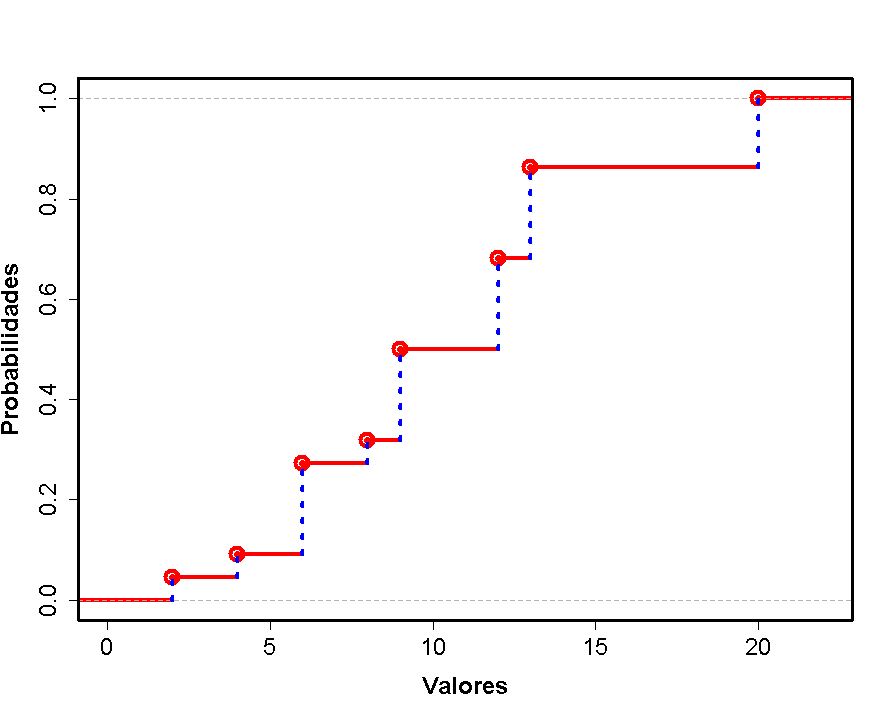
\includegraphics[height=8cm]{../fig/Cap04-FuncionDistribucionVariableAleatoria.png}
	\end{enColor}
	\begin{bn}
    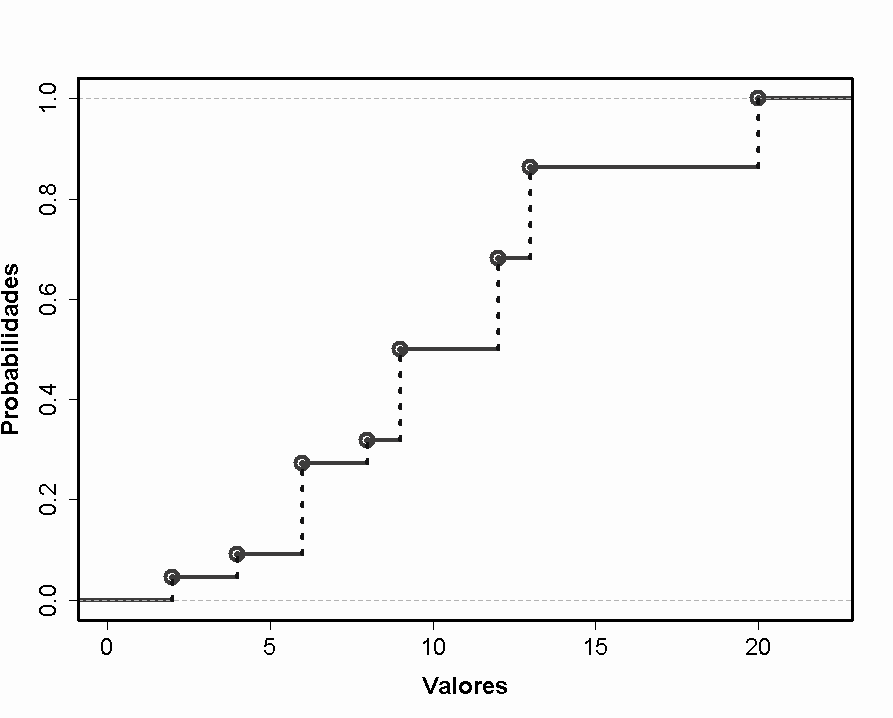
\includegraphics[height=8cm]{../fig/Cap04-FuncionDistribucionVariableAleatoria-bn.png}
	\end{bn}
	\caption{Una ``típica'' función de distribución de una variable aleatoria discreta}
	\label{cap04:fig:GraficaFuncionDistribucionVariableAleatoriaDiscreta}
    \end{figure}

\subsection{Cuantiles de una variable aleatoria discreta.}
\label{cap04:subsec:CuantilesVariableAleatoriaDiscreta}
%\noindent{\bf Opcional: puede omitirse en una primera lectura.}\\
La Figura \ref{cap04:fig:GraficaFuncionDistribucionVariableAleatoriaDiscreta} (pág. \pageref{cap04:fig:GraficaFuncionDistribucionVariableAleatoriaDiscreta}) ayuda a entender que, si fijamos una probabilidad $p_0$ cualquiera, cuanto tratemos de resolver la siguiente ecuación en $x$:
\[F(x)=p_0\]
la mayor parte de las veces no podremos encontrar una solución. No hay solución, salvo que $p_0$ sea $0$, o uno de los valores $p_1$, $p_1+p_2$, \ldots, $1$, que definen la altura de los peldaños. Mencionamos esto aquí como advertencia,  porque cuando estudiemos las variables aleatorias continuas, veremos que allí la situación es distinta y ese tipo de ecuaciones siempre tienen solución. En el caso que ahora nos ocupa, el de las variables aleatorias discretas, con un número finito de valores como la de la Tabla \ref{cap04:tabla:tablaDistribucionProbabilidadGenericaVariableAleatoriaDiscreta}, tenemos que aprender a ser más cautos cuando trabajamos con la función de distribución $F$. De momento nos conformamos con la advertencia, pero profundizaremos más en las consecuencias de este hecho más adelante. Concretamente, en el Capítulo \ref{cap:TeoremaCentralLimite}, al hacer inferencia para la Distribución Binomial, cuando esta discusión se convertirá en un problema más acuciante.
%    \begin{figure}[b!]
%	\centering
%	\begin{enColor}
%    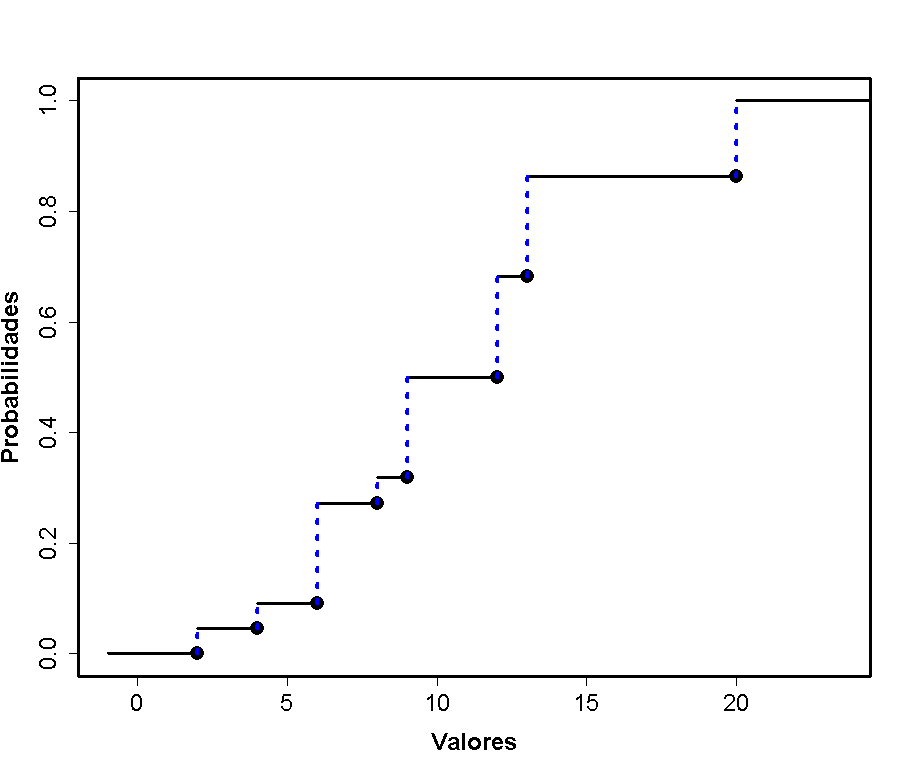
\includegraphics[height=8cm]{../fig/Cap04-PseudoFuncionDistribucionVariableAleatoria.png}
%	\end{enColor}
%	\begin{bn}
%    \includegraphics[height=8cm]{../fig/Cap04-PseudoFuncionDistribucionVariableAleatoria-bn.png}
%	\end{bn}
%	\caption{Usando $<$ en lugar de $\leq$ al acumular la probabilidad de una variable aleatoria discreta}
%	\label{cap04:fig:GraficaPseudoFuncionDistribucionVariableAleatoriaDiscreta}
%    \end{figure}

Puesto que la igualdad $F(x)=p_0$ puede no tener solución, lo que haremos, dada una probabilidad  $p_0$, es considerar la desigualdad
\[F(x)\geq p_0\]
La Figura \ref{cap04:fig:GraficaFuncionDistribucionVariableAleatoriaDiscreta} ayuda a entender que, sea cual sea la probabilidad $p_0$ entre $0$ y $1$, esa desigualdad tiene solución. La dificultad, ahora, es que tiene demasiadas, porque $F$ es constante por intervalos. Es decir, $F$ vale lo mismo para todos los $x$ que quedan debajo de cada uno de los peldaños de la Figura \ref{cap04:fig:GraficaFuncionDistribucionVariableAleatoriaDiscreta}. La solución es utilizar el extremo izquierdo de esos intervalos. Concretamente, la definición es esta:
    \begin{center}
    \fcolorbox{black}{Gris025}{
    \begin{minipage}{12cm}
        \begin{center}
        {\bf Cuantil $p_0$ de una variable aleatoria discreta}
        \index{cuantil de una variable aleatoria discreta}
        \end{center}
        Si $X$ es una variable aleatoria discreta, cuya función de distribución es $F(x)$, entonces, dada una probabilidad $p_0$ cualquiera, el {\sf cuantil} $p_0$ de $X$ es {\bf el menor valor} $x^*$ (técnicamente, el ínfimo de los $x^*$) que cumple:
        \begin{equation}
        \label{cap04:ecu:CuantilVariableAleatoriaDiscreta}
            F(x^*)\geq p_0.
        \end{equation}
    \end{minipage}}
    \end{center}
%Hemos definido la función de distribución usando la desigualdad $\leq$. Si usamos la desigualdad estricta $<$, para  definir otra función:
%\[H(x)=P(X < x )\]
%la gráfica en escalera que se obtiene es similar, como muestra la Figura \ref{cap04:fig:GraficaPseudoFuncionDistribucionVariableAleatoriaDiscreta}, sólo que ahora los puntos sólidos {\em ``han caído''} al segmento inferior, ocupando su extremo derecho. En particular, usando esas dos figuras como ayuda, se comprende que, dada cualquier probabilidad $p_0$, existe un único valor $x^*$ (de entre los valores que toma la variable aleatoria $X$) tal que
%\[H(x^*) < p_0 \leq F(x^*).\]
%Para verlo imagínate un segmento horizontal, situado a altura $p_0$, que recorre de abajo a arriba el intervalo $[0,1]$. En cualquier momento, el segmento está entre uno de los puntos situados en el extremo derecho de un segmento de la Figura \ref{cap04:fig:GraficaPseudoFuncionDistribucionVariableAleatoriaDiscreta}, y el punto situado justo encima, en el extremo izquierdo de uno de los intervalos en la Figura \ref{cap04:fig:GraficaFuncionDistribucionVariableAleatoriaDiscreta}. Esos dos puntos están situados ambos sobre el valor $x^*$ del eje de abscisas.
%
%Este valor $x^*$ es el {\sf cuantil} $p_0$\index{cuantil de una variable aleatoria discreta} de la variable $X$. Otra manera equivalente de definirlo es diciendo que el $x^*$ es el {\em menor valor} para el que se cumple
%\[F(x^*) \geq p_0,\]
%y mientras $p_0$ sea una probabilidad, siempre existe ese valor $x^*$.
Así que, remitiéndonos de nuevo a la Figura \ref{cap04:fig:GraficaFuncionDistribucionVariableAleatoriaDiscreta}, los cuantiles son las coordenadas $x$ de los puntos sólidos que aparecen en los extremos izquierdos de los segmentos horizontales, en esa figura. Por supuesto, coinciden con los valores $x_1$,\ldots,$x_k$ que toma la variable aleatoria $X$. La parte más interesante de la definición de cuantil es la correspondencia que establecemos de probabilidades a valores:
\[ \mbox{Probabilidad } p_0   \dashrightarrow x_i, \mbox{ el valor que es el cuantil de }p_0, \]
Esta correspondencia es, de alguna forma, la correspondencia inversa de la asignación
\[ \mbox{ valor }x \dashrightarrow \mbox{ probabilidad acumulada }F(x)\]
que hace la función de distribución $F$. Y decimos ``de alguna manera'' porque el camino:
\[
    (\mbox{ valor } x)\,\dashrightarrow\, (\mbox{probabilidad }p_0=F(x))\,\dashrightarrow (\mbox{ cuantil de }p_0)
\]
en la mayoría de los casos no nos llevará de vuelta al valor $x$  con el que hemos comenzado, sino al valor más cercano a $x$, por la izquierda, de entre los valores $x_1$,\ldots,$x_k$ que toma la variable $X$. La Figura \ref{cap04:fig:GraficaFuncionDistribucionVariableAleatoriaDiscreta} puede ayudar a entender esto. Y veremos ejemplos más adelante, al tratar sobre la Distribución Binomial en el Capítulo \ref{cap:TeoremaCentralLimite}.



\section{Independencia y vectores aleatorios discretos.}
\label{cap04:sec:IndependenciaVariablesAleatoriasDiscretas}
\noindent{\bf Opcional: esta sección puede omitirse en una primera lectura.}\\

%El contenido de esta sección no es imprescindible para seguir adelante en el curso. Por otra parte, la discusión es necesariamente más técnica, y puede que requiera del lector un esfuerzo adicional que tal vez sea mejor reservar, para el momento en que se haya ganado algo más de confianza con los conceptos de este capítulo. Así que la sección puede omitirse en una primera lectura. No obstante, hemos preferido mantenerla en este capítulo, porque es su sitio natural (o porque no sabríamos donde ponerla, de otra manera...)

Ya sabemos lo que significa que dos sucesos sean independientes. Y ahora vamos a tratar de extender esa misma noción de independencia a las variables aleatorias. La idea intuitiva es la misma. Dos variables aleatorias, $X$ e $Y,$ serán independientes si el conocimiento que tenemos sobre el valor de $X$ no afecta de ninguna manera al que tenemos sobre el valor de $Y$.

Esa idea informal está muy bien, pero ya vimos en su momento que cuando tratábamos de concretarlo, en el caso de los sucesos, necesitábamos la noción de probabilidad condicionada que, a su vez, descansa, en última instancia, sobre la {\em intersección} de los sucesos. La intersección es lo que ambos sucesos tienen en común. Es algo que caracteriza {\em conjuntamente} a la pareja formada por dos sucesos.

Para poder llevar esa misma idea al caso de dos variables aleatorias $X$ e $Y$ vamos a tener que aprender a pensar también en ambas variables {\em conjuntamente}. Esto puede parecer complicado. Pero, de hecho, al igual que sucede con la probabilidad condicionada, a menudo resulta más sencillo trabajar con las propiedades conjuntas de dos variables, que tratar de hacerlo por separado.  {!`}Especialmente cuando son dependientes, claro!

Vamos a pensar entonces en la pareja formada por las variables $X$ e $Y$, y para representar esa pareja usaremos la notación $(X,Y)$. El trabajo que vamos a hacer en este apartado se extiende con relativa facilidad al caso de $k$ variables aleatorias, pensadas conjuntamente, como un objeto que se representa
\[(X_1,\ldots,X_k).\]
Esta clase de objetos se llaman a menudo {\sf vectores aleatorios}\index{vector aleatorio} (en inglés, {\em random vector}\index{random vector}). El número de componentes $k$ es la {\sf dimensión} del vector aleatorio; de manera que, por ejemplo, $(X,Y)$ será un vector aleatorio bidimensional. Un vector aleatorio $(X,Y)$ que sólo toma una cantidad finita de valores es un {\sf vector aleatorio discreto}\index{vector aleatorio discreto}.

Ya hemos visto que una variable aleatoria $X$ queda caracterizada por su tabla o función de densidad (ver pág. \pageref{cap04:ecu:funcionDensidadVariableAleatoriaDiscreta}). Esa tabla nos dice, para cada uno de los valores $x_i$ que puede tomar la variable, cuál es la probabilidad $p_i$ de que $X$ tome ese valor. Cuando se trata de una pareja $(X,Y)$ existe un objeto análogo, que es la función de densidad conjunta de $X$ e $Y$.
    \begin{center}
    \fcolorbox{black}{Gris025}{
    \begin{minipage}{12cm}
        \begin{center}
        {\bf Función de densidad conjunta de un vector aleatorio discreto.}
        \end{center}
        \index{función de densidad conjunta de un vector aleatorio discreto}
        Si $(X, Y)$ es un vector aleatorio discreto, que sólo toma una cantidad finita de valores,        su {\sf función de densidad conjunta} es la función definida mediante:
        \begin{equation}
        \label{cap04:ecu:FuncionDensidadConjuntaVectorAleatorio}
        f(x,y)=P\bigg((X, Y) =(x, y)\bigg) = P(X=x, Y=y).
        \end{equation}
        (Hemos usado dos notaciones para intentar aclarar la definición. La segunda es la más habitual.) Es decir, la función $f$ nos dice cuál es la probabilidad de que el vector $(X,Y)$ tome el valor $(x,y)$. Al ser $(X,Y)$ discreto, sólo existe una cantidad finita de parejas $(x,y)$ para las que esta probabilidad es distinta de $0$.
    %\end{definicion}
    \end{minipage}}
    \end{center}
\quad\\
Veamos un primer ejemplo sencillo, con variables que ya hemos encontrado antes.
\begin{ejemplo}
\label{cap04:ejem:VectoAleatorioDiscretoDado}
En el Ejemplo \ref{cap04:ejem:varianzaSumaVariablesAleatoriasDiscretas} hemos dejado pendiente la cuestión de si, en el caso del lanzamiento de dos dados, las variables $X$ (suma) e $Y$ (diferencia, en valor absoluto) son o no independientes. Todavía tenemos que definir lo que significa la independencia en este contexto. En el Ejemplo \ref{cap04:ejem:IndependenciaVariablesAleatoriasDiscretas} volveremos sobre esa cuestión. Ahora, para preparar el terreno, vamos a construir la tabla o función de densidad conjunta de ambas variables. Para ayudarnos a ver cuál es esa tabla vamos a pensar en el espacio muestral formado por los $36$ posibles resultados al lanzar dos dados. La parte (a) de la Tabla \ref{cap04:tabla:VectoAleatorioDiscretoDado} (pág. \pageref{cap04:tabla:VectoAleatorioDiscretoDado}) muestra en cada fila uno de esos $36$ resultados, y para cada resultado se muestran, en las dos últimas columnas de la tabla, los valores de $X$ e $Y$.

Esas dos últimas columnas nos proporcionan la información que necesitamos sobre la densidad conjunta del vector $(X,Y)$. Tenemos 36 pares de valores $(X, Y)$, pero que no son todos distintos los unos de los otros. Después de ver cuántos pares distintos hay, y cuántas veces aparece cada uno de ellos, la parte (b) de la la Tabla \ref{cap04:tabla:VectoAleatorioDiscretoDado} usa esa información para mostrar la probabilidad de aparición de cada uno de esos pares. Esa tabla describe, por tanto, la función de densidad conjunta del vector $(X, Y)$. Y nos dice, por ejemplo, que
\[f(5,3) = P(X=5, Y=3) = \dfrac{2}{36}.\]
Si quieres, puedes buscar en la parte (a) de la tabla cuales son los dos puntos del espacio muestral que corresponden a este resultado. Fíjate, en la parte (b) de la Tabla \ref{cap04:tabla:VectoAleatorioDiscretoDado} en que, aunque $X$ puede tomar el valor $6$, e $Y$ puede tomar el valor $1$, para la densidad conjunta es $f(6,1)=0$.

\begin{table}[p]
\begin{center}
\begin{tabular}{cc}
(a) & (b)\\[5mm]
{\scriptsize
\begin{tabular}{|c|c|c|c|}
  \hline
dado1 & dado2 & X & Y \\
  \hline
  1 &   1 &   2 &   0 \\ \hline
    2 &   1 &   3 &   1 \\ \hline
    3 &   1 &   4 &   2 \\ \hline
    4 &   1 &   5 &   3 \\ \hline
    5 &   1 &   6 &   4 \\ \hline
    6 &   1 &   7 &   5 \\ \hline
    1 &   2 &   3 &   1 \\ \hline
    2 &   2 &   4 &   0 \\ \hline
    3 &   2 &   5 &   1 \\ \hline
    4 &   2 &   6 &   2 \\ \hline
    5 &   2 &   7 &   3 \\ \hline
    6 &   2 &   8 &   4 \\ \hline
    1 &   3 &   4 &   2 \\ \hline
    2 &   3 &   5 &   1 \\ \hline
    3 &   3 &   6 &   0 \\ \hline
    4 &   3 &   7 &   1 \\ \hline
    5 &   3 &   8 &   2 \\ \hline
    6 &   3 &   9 &   3 \\ \hline
    1 &   4 &   5 &   3 \\ \hline
    2 &   4 &   6 &   2 \\ \hline
    3 &   4 &   7 &   1 \\ \hline
    4 &   4 &   8 &   0 \\ \hline
    5 &   4 &   9 &   1 \\ \hline
    6 &   4 &  10 &   2 \\ \hline
    1 &   5 &   6 &   4 \\ \hline
    2 &   5 &   7 &   3 \\ \hline
    3 &   5 &   8 &   2 \\ \hline
    4 &   5 &   9 &   1 \\ \hline
    5 &   5 &  10 &   0 \\ \hline
    6 &   5 &  11 &   1 \\ \hline
    1 &   6 &   7 &   5 \\ \hline
    2 &   6 &   8 &   4 \\ \hline
    3 &   6 &   9 &   3 \\ \hline
    4 &   6 &  10 &   2 \\ \hline
    5 &   6 &  11 &   1 \\ \hline
    6 &   6 &  12 &   0 \\
   \hline
\end{tabular}
}
&
\begin{tabular}[b]{c|r|r|r|r|r|r|r|}
  \multicolumn{1}{c}{}&\multicolumn{1}{c}{}&\multicolumn{6}{c}{Valor de $Y$}\\
  \cline{3-8}
  \multicolumn{1}{c}{}
  && 0 & 1 & 2 & 3 & 4 & 5 \\  \cline{2-8}
  \multirow{10}{*}{
  \rotatebox{90}{Valor de $X$}
  }
    &   2 & 1/36 & 0 & 0 & 0 & 0 & 0 \\ \cline{2-8}
    &   3 & 0 & 1/18 & 0 & 0 & 0 & 0 \\ \cline{2-8}
    &   4 & 1/36 & 0 & 1/18 & 0 & 0 & 0 \\ \cline{2-8}
    &   5 & 0 & 1/18 & 0 & 1/18 & 0 & 0 \\ \cline{2-8}
    &   6 & 1/36 & 0 & 1/18 & 0 & 1/18 & 0 \\ \cline{2-8}
    &   7 & 0 & 1/18 & 0 & 1/18 & 0 & 1/18 \\ \cline{2-8}
    &   8 & 1/36 & 0 & 1/18 & 0 & 1/18 & 0 \\ \cline{2-8}
    &   9 & 0 & 1/18 & 0 & 1/18 & 0 & 0 \\ \cline{2-8}
    &   10 & 1/36 & 0 & 1/18 & 0 & 0 & 0 \\ \cline{2-8}
    &   11 & 0 & 1/18 & 0 & 0 & 0 & 0 \\ \cline{2-8}
    &   12 & 1/36 & 0 & 0 & 0 & 0 & 0 \\
   \cline{2-8}
\end{tabular}
\end{tabular}

%(a)\\[3mm]
%{\scriptsize
%\begin{tabular}{|c|c|c|c|}
%  \hline
%dado1 & dado2 & X & Y \\
%  \hline
%  1 &   1 &   2 &   0 \\ \hline
%    2 &   1 &   3 &   1 \\ \hline
%    3 &   1 &   4 &   2 \\ \hline
%    4 &   1 &   5 &   3 \\ \hline
%    5 &   1 &   6 &   4 \\ \hline
%    6 &   1 &   7 &   5 \\ \hline
%    1 &   2 &   3 &   1 \\ \hline
%    2 &   2 &   4 &   0 \\ \hline
%    3 &   2 &   5 &   1 \\ \hline
%    4 &   2 &   6 &   2 \\ \hline
%    5 &   2 &   7 &   3 \\ \hline
%    6 &   2 &   8 &   4 \\ \hline
%    1 &   3 &   4 &   2 \\ \hline
%    2 &   3 &   5 &   1 \\ \hline
%    3 &   3 &   6 &   0 \\ \hline
%    4 &   3 &   7 &   1 \\ \hline
%    5 &   3 &   8 &   2 \\ \hline
%    6 &   3 &   9 &   3 \\ \hline
%    1 &   4 &   5 &   3 \\ \hline
%    2 &   4 &   6 &   2 \\ \hline
%    3 &   4 &   7 &   1 \\ \hline
%    4 &   4 &   8 &   0 \\ \hline
%    5 &   4 &   9 &   1 \\ \hline
%    6 &   4 &  10 &   2 \\ \hline
%    1 &   5 &   6 &   4 \\ \hline
%    2 &   5 &   7 &   3 \\ \hline
%    3 &   5 &   8 &   2 \\ \hline
%    4 &   5 &   9 &   1 \\ \hline
%    5 &   5 &  10 &   0 \\ \hline
%    6 &   5 &  11 &   1 \\ \hline
%    1 &   6 &   7 &   5 \\ \hline
%    2 &   6 &   8 &   4 \\ \hline
%    3 &   6 &   9 &   3 \\ \hline
%    4 &   6 &  10 &   2 \\ \hline
%    5 &   6 &  11 &   1 \\ \hline
%    6 &   6 &  12 &   0 \\
%   \hline
%\end{tabular}
%}\\[3mm]
%(b)\\[3mm]
%\begin{tabular}{rllllll}
%  \hline
% & 0 & 1 & 2 & 3 & 4 & 5 \\
%  \hline
%2 & 1/36 & 0 & 0 & 0 & 0 & 0 \\
%  3 & 0 & 1/18 & 0 & 0 & 0 & 0 \\
%  4 & 1/36 & 0 & 1/18 & 0 & 0 & 0 \\
%  5 & 0 & 1/18 & 0 & 1/18 & 0 & 0 \\
%  6 & 1/36 & 0 & 1/18 & 0 & 1/18 & 0 \\
%  7 & 0 & 1/18 & 0 & 1/18 & 0 & 1/18 \\
%  8 & 1/36 & 0 & 1/18 & 0 & 1/18 & 0 \\
%  9 & 0 & 1/18 & 0 & 1/18 & 0 & 0 \\
%  10 & 1/36 & 0 & 1/18 & 0 & 0 & 0 \\
%  11 & 0 & 1/18 & 0 & 0 & 0 & 0 \\
%  12 & 1/36 & 0 & 0 & 0 & 0 & 0 \\
%   \hline
%\end{tabular}
%{\small
%\begin{tabular}{l|c|c|c|c|c|c|c|c|c|c|c|c|}
%  \multicolumn{2}{c}{}
%  &\multicolumn{11}{c}{Valor de $X$}\\
%  \cline{3-13}
%
%  \multicolumn{2}{c|}{}
% & 2 & 3 & 4 & 5 & 6 & 7 & 8 & 9 & 10 & 11 & 12 \\
%  \cline{2-13}
%\multirow{6}{*}{
%\begin{minipage}{0.8cm}
%{\small
%Valor\\ de $Y$
%}
%\end{minipage}
%}
%& 0 &   $1/36$ &   0 &   $1/36$ &   0 &   $1/36$ &   0 &   $1/36$ &   0 &   $1/36$ &   0 &   $1/36$ \\ \cline{2-13}
%&  1 &   0 &   $2/36$ &   0 &   $2/36$ &   0 &   $2/36$ &   0 &   $2/36$ &   0 &   $2/36$ &   0 \\ \cline{2-13}
%&  2 &   0 &   0 &   $2/36$ &   0 &   $2/36$ &   0 &   $2/36$ &   0 &   $2/36$ &   0 &   0 \\ \cline{2-13}
%&  3 &   0 &   0 &   0 &   $2/36$ &   0 &   $2/36$ &   0 &   $2/36$ &   0 &   0 &   0 \\ \cline{2-13}
%&  4 &   0 &   0 &   0 &   0 &   $2/36$ &   0 &   $2/36$ &   0 &   0 &   0 &   0 \\ \cline{2-13}
%&  5 &   0 &   0 &   0 &   0 &   0 &   $2/36$ &   0 &   0 &   0 &   0 &   0 \\
%   \cline{2-13}
%\end{tabular}
%}
\end{center}
\caption{Ejemplo \ref{cap04:ejem:VectoAleatorioDiscretoDado}. (a) Los valores de $X$ e $Y$ en cada punto del espacio muestral. (b) La tabla de densidad conjunta de $X$ e $Y$.}
\label{cap04:tabla:VectoAleatorioDiscretoDado}
\end{table}
Algunas preguntas en las que puedes ir pensando:
\begin{enumerate}
  \item ¿Cuánto vale la suma de todos los elementos de la Tabla \ref{cap04:tabla:VectoAleatorioDiscretoDado}(b)?
  \item Usando la la Tabla \ref{cap04:tabla:VectoAleatorioDiscretoDado}(b) (y sólo esa tabla) ¿cómo calcularías la probabilidad de que $Y$ tome el valor $2$ (sea cual sea el valor de $X$)?
  \item ¿Crees (intuitivamente) que $X$ e $Y$, en este ejemplo, son independientes?
\end{enumerate}
Volveremos sobre estas preguntas en breve.
\qed
\end{ejemplo}

\subsubsection{Aclaraciones sobre la representación como tabla o como función de la densidad conjunta.}

En el Ejemplo \ref{cap04:ejem:VectoAleatorioDiscretoDado} hemos visto una forma bastante habitual de presentar la tabla de densidad conjunta de un vector aleatorio $(X,Y)$. Si $X$ toma los valores $x_1,\ldots,x_k$, mientras que $Y$ toma los valores $y_1,\ldots,y_m$, entonces podemos hacer una tabla de doble entrada, como la Tabla \ref{cap04:tabla:DensidadConjuntaVectorAleatorioDiscreto}
\begin{table}[h!]
\[
\hspace{-1cm}\mbox{Valor de $X$}\quad\begin{array}{|c|c|c|c|c|}
\multicolumn{1}{c}{} &\multicolumn{4}{c}{\mbox{Valor de $Y$}}{}\\
\cline{2-5}
\multicolumn{1}{c|}{} &y_1    & y_2   & \cdots    & y_m\\
    \hline
x_1 &p_{11} & p_{12}& \cdots    & p_{1m}\\
    \hline
x_2 &p_{21} & p_{22}& \cdots    & p_{2m}\\
\hline
\vdots&     &       & \ddots    &       \\
    \hline
x_k &p_{k1} & p_{k2}& \cdots    & p_{km}\\
    \hline
\end{array}
\]
\caption{Tabla de densidad conjunta de probabilidad para un vector aleatorio discreto $(X,Y)$.}
\label{cap04:tabla:DensidadConjuntaVectorAleatorioDiscreto}
\end{table}
en la que $f(x_i,y_j)=p_{ij}$. Naturalmente, como muestra el ejemplo, puede haber pares $(x_i,y_j)$ tales que $f(x_i,y_j)=0$, aunque las probabilidades $P(X=x_i)$ y $P(y=y_j)$ sean ambas no nulas.

Una aclaración más, para evitar posibles confusiones: cuando decimos que $X$ toma los valores $x_1,\ldots,x_k$, queremos decir que si $x_0$ {\em no} es uno de los valores $x_1,\ldots,x_k$, entonces, sea cual sea el valor de $y_0$, se cumple {\em automáticamente:}
\[
f(x_0,y_0)=0.
\]
Y lo mismo sucede si $y_0$ no es uno de los valores $y_1,\ldots,y_m$. Entonces, sea cual sea $x_0$, la densidad conjunta $f(x_0,y_0)$ es automáticamente nula.

\noindent Por si estás cansado de ejemplos con dados (paciencia, aún nos quedan unos cuantos en el curso...), hemos incluido otro ejemplo, que puedes encontrar más interesante.
\begin{ejemplo}
\label{cap04:ejem:vectorAleatorioDias2014}
Imagínate que el departamento de control de calidad de una gran empresa quiere realizar un estudio sobre su servicio de atención al cliente, para saber si los recursos asignados a ese servicio son suficientes. Si la empresa es grande, puede que el servicio haya atendido decenas de miles de peticiones a lo largo de un año. Y puede resultar poco práctico tratar de analizarlas todas. Para hacerse una idea rápida, se podrían seleccionar  al azar $30$ días del año, y analizar el funcionamiento del servicio en esos días. Ya volveremos sobre estas ideas más adelante, pero el hecho de seleccionar los días al azar es esencial, para garantizar que el conjunto de días seleccionados  es {\em representativo} y reducir la posible influencia de factores desconocidos. Por ejemplo si todos los días seleccionados fueran viernes o si se seleccionan varios días en los que hubo grandes averías del servicio telefónico, la muestra no sería representativa. La selección al azar hace muy improbable elegir una muestra así.   

Para llevar adelante este plan, por tanto, tenemos que seleccionar un día del año al azar. Y después, cuando analicemos los resultados, querremos saber si ese día es laborable, si es viernes o jueves, etc.  Así que vamos a pensar en un experimento en el que elegimos al azar un día del año 2014. Este es el mecanismo básico. Luego bastaría con repetirlo para obtener los 30 días necesarios. Volveremos sobre esto en el Capítulo \ref{cap:IntervalosConfianza}, cuando hablemos de muestreo.

Vamos a considerar el vector aleatorio $(X,Y)$, donde el valor de $X$ indica el día de la semana (desde $1$ para lunes, a $7$ para domingo) , y el valor de $Y$ indica el día del mes. La Tabla \ref{cap04:tabla:vectorAleatorioDias2014} (pág. \pageref{cap04:tabla:vectorAleatorioDias2014}) es una tabla de {\em frecuencia} conjunta de $X$ e $Y$.  No hemos presentado directamente la tabla de densidad conjunta porque creemos que en este caso es más fácil visualizar los datos en forma de frecuencias, y porque el cálculo  de las probabilidades a partir de ahí es inmediato: para conseguir la tabla de densidad del vector aleatorio $(X,Y)$ basta con dividir cada elemento de la Tabla \ref{cap04:tabla:vectorAleatorioDias2014} por $365$.

Para entender más a fondo el ejemplo, veamos cuanto vale
\[f(4, 20) = P(X=4, Y=20).\]
Vamos a la Tabla \ref{cap04:tabla:vectorAleatorioDias2014} y comprobamos que la frecuencia del valor $(X,Y)=(4,20)$ es $3$. Por lo tanto:
\[f(4, 20) = P(X=4, Y=20)=\dfrac{3}{365}.\]
Esto significa que si elegimos un día al azar  del año $2014$, la probabilidad de que sea $X=4$ (el día es jueves) e $Y=20$ (el día elegido es el día $20$ del mes) es de $\frac{3}{365}\approx 0.008219$.

\begin{table}[p]
\centering
$Y=$ día del mes
\begin{tabular}{|r|r|r|r|r|r|r|r|}

  \multicolumn{1}{c}{}&\multicolumn{7}{ c }{$X=$ día de la semana.} \\
  \cline{2-8}
 \multicolumn{1}{c|}{}& 1 & 2 & 3 & 4 & 5 & 6 & 7 \\
  \hline
1 &   2 &   2 &   2 &   1 &   1 &   3 &   1 \\
  2 &   1 &   2 &   2 &   2 &   1 &   1 &   3 \\
  3 &   3 &   1 &   2 &   2 &   2 &   1 &   1 \\
  4 &   1 &   3 &   1 &   2 &   2 &   2 &   1 \\
  5 &   1 &   1 &   3 &   1 &   2 &   2 &   2 \\
  6 &   2 &   1 &   1 &   3 &   1 &   2 &   2 \\
  7 &   2 &   2 &   1 &   1 &   3 &   1 &   2 \\
  8 &   2 &   2 &   2 &   1 &   1 &   3 &   1 \\
  9 &   1 &   2 &   2 &   2 &   1 &   1 &   3 \\
  10 &   3 &   1 &   2 &   2 &   2 &   1 &   1 \\
  11 &   1 &   3 &   1 &   2 &   2 &   2 &   1 \\
  12 &   1 &   1 &   3 &   1 &   2 &   2 &   2 \\
  13 &   2 &   1 &   1 &   3 &   1 &   2 &   2 \\
  14 &   2 &   2 &   1 &   1 &   3 &   1 &   2 \\
  15 &   2 &   2 &   2 &   1 &   1 &   3 &   1 \\
  16 &   1 &   2 &   2 &   2 &   1 &   1 &   3 \\
  17 &   3 &   1 &   2 &   2 &   2 &   1 &   1 \\
  18 &   1 &   3 &   1 &   2 &   2 &   2 &   1 \\
  19 &   1 &   1 &   3 &   1 &   2 &   2 &   2 \\
  20 &   2 &   1 &   1 &   3 &   1 &   2 &   2 \\
  21 &   2 &   2 &   1 &   1 &   3 &   1 &   2 \\
  22 &   2 &   2 &   2 &   1 &   1 &   3 &   1 \\
  23 &   1 &   2 &   2 &   2 &   1 &   1 &   3 \\
  24 &   3 &   1 &   2 &   2 &   2 &   1 &   1 \\
  25 &   1 &   3 &   1 &   2 &   2 &   2 &   1 \\
  26 &   1 &   1 &   3 &   1 &   2 &   2 &   2 \\
  27 &   2 &   1 &   1 &   3 &   1 &   2 &   2 \\
  28 &   2 &   2 &   1 &   1 &   3 &   1 &   2 \\
  29 &   2 &   2 &   2 &   1 &   1 &   2 &   1 \\
  30 &   1 &   2 &   2 &   2 &   1 &   1 &   2 \\
  31 &   1 &   0 &   1 &   1 &   2 &   1 &   1 \\
   \hline
\end{tabular}
\caption{Tabla de frecuencia conjunta de $X$ (día de la semana) e $Y$ día del mes, para el año 2014, en el Ejemplo \ref{cap04:ejem:vectorAleatorioDias2014}.}
\label{cap04:tabla:vectorAleatorioDias2014}
\end{table}
\qed
\end{ejemplo}


\subsection{Densidades marginales.}
\label{cap04:subsec:DendidadesMarginales}

Recuerda que dos sucesos $A$ y $B$ son independientes si se cumple:
\[P(A\cap B)= P(A)\cdot P(B).\]
Ahora queremos trasladar esta definición al caso de un vector aleatorio discreto. La densidad conjunta, que ya hemos definido, va a jugar el papel que  la intersección jugaba en el caso de los sucesos. Pero entonces necesitamos algo que juegue el papel de las probabilidades {\em por separado} de cada una de las componentes $X$ e $Y$ del vector aleatorio. Ese papel lo juegan las densidades marginales.
    \begin{center}
    \fcolorbox{black}{Gris025}{
    \begin{minipage}{12cm}
        \begin{center}
        {\bf Densidades marginales de un vector aleatorio discreto.}
        \end{center}
        Sea $(X, Y)$ es un vector aleatorio discreto, con función de densidad $f$. Supongamos que
        $X$ toma los valores $x_1,\ldots,x_k$ e $Y$ toma los valores $y_1,\ldots,y_m$, en el sentido que hemos precisado antes. Entonces la {\sf función de densidad marginal}\index{función de densidad marginal (caso discreto)}\index{marginal, función de densidad (caso discreto)}\index{densidad marginal, función de (caso discreto)} (en inglés, {\em marginal density}\index{marginal density}) de $X$ es la función definida mediante:
        \begin{equation}
        \label{cap04:ecu:FuncionDensidadMarginalXVectorAleatorio}
        f_X(x)=f(x,y_1)+ f(x,y_2)+\cdots+f(x,y_m)=\underbrace{
        \sum_{j=1}^m f(x, y_j).}_{\mbox{\tiny todos los valores de $y$}}
        \end{equation}
        De la misma forma, la función de densidad marginal de $Y$ es
        \begin{equation}
        \label{cap04:ecu:FuncionDensidadMarginalYVectorAleatorio}
        f_Y(y)=f(x_1,y)+ f(x_2,y)+\cdots+f(x_k,y)=\underbrace{
        \sum_{i=1}^k f(x_i, y).}_{\mbox{\tiny todos los valores de $x$}}
        \end{equation}
    \end{minipage}}
    \end{center}
Como hemos indicado, la densidad marginal de $X$,  para un valor $x$ dado, se obtiene manteniendo fijo ese valor de $x$ y sumando sobre todos los posibles valores de $Y$. La densidad marginal de $Y$ se define igual, intercambiando los papeles de $X$ e $Y$. Veamos un ejemplo.

\begin{ejemplo}
\label{cap04:ejem:densidadesMarginales}
{\bf (Continuación del Ejemplo \ref{cap04:ejem:VectoAleatorioDiscretoDado}, pág. \pageref{cap04:ejem:VectoAleatorioDiscretoDado}).} En la Tabla \ref{cap04:tabla:MarginalesVectoAleatorioDiscretoDado} se muestra el resultado que se obtiene si, partiendo de la Tabla \ref{cap04:tabla:VectoAleatorioDiscretoDado}(b), se suman los valores de cada fila y cada columna, y se colocan en los márgenes de la tabla. Como puede verse, el resultado es que la última columna y la última fila muestran, respectivamente, las densidades marginales de $X$ e $Y$.
\begin{table}[ht]
\begin{center}
{
\rotatebox{90}{Valor de $X$\phantom{12345}}
}
\quad
\begin{tabular}{|r|r|r|r|r|r|r|r|}
  \multicolumn{1}{c}{}&\multicolumn{7}{c}{Valor de $Y$}\\
  \cline{2-8}
  \multicolumn{1}{c|}{}& 0 & 1 & 2 & 3 & 4 & 5 & Suma \\
  \hline
  2 & 1/36 & 0 & 0 & 0 & 0 & 0 & 1/36 \\ \hline
  3 & 0 & 1/18 & 0 & 0 & 0 & 0 & 1/18 \\ \hline
  4 & 1/36 & 0 & 1/18 & 0 & 0 & 0 & 1/12 \\ \hline
  5 & 0 & 1/18 & 0 & 1/18 & 0 & 0 & 1/9 \\ \hline
  6 & 1/36 & 0 & 1/18 & 0 & 1/18 & 0 & 5/36 \\ \hline
  7 & 0 & 1/18 & 0 & 1/18 & 0 & 1/18 & 1/6 \\ \hline
  8 & 1/36 & 0 & 1/18 & 0 & 1/18 & 0 & 5/36 \\ \hline
  9 & 0 & 1/18 & 0 & 1/18 & 0 & 0 & 1/9 \\ \hline
  10 & 1/36 & 0 & 1/18 & 0 & 0 & 0 & 1/12 \\ \hline
  11 & 0 & 1/18 & 0 & 0 & 0 & 0 & 1/18 \\ \hline
  12 & 1/36 & 0 & 0 & 0 & 0 & 0 & 1/36 \\ \hline
  Suma & 1/6 & 5/18 & 2/9 & 1/6 & 1/9 & 1/18 & 1 \\
   \hline
\end{tabular}
\end{center}
\caption{Densidades marginales de $X$ e $Y$ para el vector aleatorio del Ejemplo \ref{cap04:ejem:VectoAleatorioDiscretoDado}.}
\label{cap04:tabla:MarginalesVectoAleatorioDiscretoDado}
\end{table}
\qed
\end{ejemplo}
La forma en la que se obtienen las densidades marginales a partir de la tabla de densidad conjunta explica el origen del nombre {\em marginales}; son los valores que aparecen en los márgenes de la tabla. La interpretación de las densidades marginales en términos de probabilidades es extremadamente simple, pero conviene detenerse a pensar un momento en ella:
\begin{equation}
\label{cap04:ecu:DensidadMarginalXInterpretacionProababilistica}
f_X(x)=P(X=x).
\end{equation}
La probabilidad del miembro derecho debe entenderse, en este contexto como ``la probabilidad de que se cumpla $X=x$, sin importar cuál sea el valor de $Y$''.

En el caso $n$-dimensional, la densidad marginal de $X_i$ en el vector aleatorio $(X_1,\ldots, X_n)$ se obtiene sumando sobre todas las componentes, salvo precisamente la $i$.

Para cerrar este apartado, señalaremos que las densidades marginales contienen la respuesta a las dos primeras preguntas que dejamos pendiente en el Ejemplo \ref{cap04:ejem:VectoAleatorioDiscretoDado} (pág. \pageref{cap04:ejem:VectoAleatorioDiscretoDado}).

\subsubsection{Suma total de una tabla de densidad conjunta.}

En cuanto a la primera pregunta pendiente del Ejemplo \ref{cap04:ejem:VectoAleatorioDiscretoDado}, el resultado de la celda inferior derecha de la Tabla \ref{cap04:tabla:MarginalesVectoAleatorioDiscretoDado} anticipa la respuesta. Puesto que, en última instancia, estamos estudiando la probabilidad de todos los valores posibles, las tablas de densidad conjunta de un vector aleatorio tienen siempre la propiedad de que la suma de todos los elementos de la tabla vale $1$. Puedes comprobar esto sumando los valores de las tablas de los Ejemplos \ref{cap04:ejem:VectoAleatorioDiscretoDado} y \ref{cap04:ejem:vectorAleatorioDias2014}. Para facilitar el trabajo, en el Tutorial04 veremos como usar el ordenador para hacer esto.

\subsubsection{Función de distribución de un vector aleatorio.}

La {\sf función de distribución de un vector aleatorio} se define de una manera similar a la de una variable aleatoria. Si $(X,Y)$ es el vector aleatorio, y $(x_0,y_0)$ es un par de valores cualesquiera, su función de distribución $F$ se define mediante:
\begin{equation}
\label{cap04:ecu:FuncionDistribucionVectorAleatorio}
F(x_0, y_0) = P(X\leq x_0, Y\leq y_0)=P\bigg((X\leq x_0)\cap(Y\leq y_0)\bigg).
\end{equation}
Hemos incluido las dos notaciones porque, aunque la de la intersección es la más precisa de las dos, la notación con la coma es la más usada, y en general no provoca errores. Las {\sf funciones de distribución marginales}\index{funciones de distribución marginales (caso discreto)} $F_X(x)$ y $F_Y(y)$ se definen como las densidades marginales, reemplazando en las Ecuaciones \ref{cap04:ecu:FuncionDensidadMarginalXVectorAleatorio} y \ref{cap04:ecu:FuncionDensidadMarginalYVectorAleatorio} (pág. \pageref{cap04:ecu:FuncionDensidadMarginalYVectorAleatorio}) la $f$ (densidad) por $F$ (distribución).


\subsection{Independencia.}
\label{cap04:subsec:IndependenciaVectorAleatorioDiscreto}

Las densidades marginales juegan el papel de {\em ``cada variable por separado''}, así que ya tenemos todos los ingredientes necesarios para la definición de independencia de un vector aleatorio.

    \begin{center}
    \fcolorbox{black}{Gris025}{
    \begin{minipage}{12cm}
    %\begin{definicion}
        \begin{center}
        {\bf Independencia de variables aleatorias discretas.}
        \end{center}
        \index{independencia de dos variables aleatorias discretas}
        Sea $(X,Y)$ un vector aleatorio discreto, con función de densidad conjunta $f(x,y)$, y con densidades marginales $f_X(x)$ y $f_Y(y)$. Las variables aleatorias discretas $X$ e $Y$ son {\sf independientes} si, sea cual sea el par de valores $(x,y)$ que se considere, se cumple:
        \begin{equation}
        \label{cap04:ecu:indepedenciaVariablesAleatoriasDiscretas}
        f(x,y)=f_X(x)\cdot f_Y(y).
        \end{equation}
        En términos de las funciones de distribución, esto es equivalente a que sea:
        \begin{equation}
        \label{cap04:ecu:indepedenciaVariablesAleatoriasDiscretasFDistribucion}
        F(x,y)=F_X(x)\cdot F_Y(y).
        \end{equation}
    %\end{definicion}
    \end{minipage}}
    \end{center}
En el caso de un vector aleatorio $n$ dimensional, como $(X_1,X_2,\ldots,X_n)$, la independencia significa que la densidad conjunta es el producto de las $n$ densidades marginales:
\begin{equation}
\label{cap04:ecu:indepedenciaVariablesAleatoriasDiscretasCasoNdimensional}
f(x_1,x_2,\ldots,x_n) = f_{X_1}(x_1)\cdot f_{X_2}(x_2)\cdot\,\cdots\,\cdot f_{X_n}(x_n)
\end{equation}
En este caso, a diferencia de lo que sucedía con la independencia de sucesos, para probar la independencia basta con esto y no es necesario considerar productos dos a dos, tres a tres, etc. Si quieres más detalles tendrás que consultar un libro de Estadística Matemática, como por ejemplo \cite{horra2003estadistica}\pedniente{Cita Shao}. 


¿Cómo se puede comprobar la independencia, a partir de la tabla de densidad conjunta? En dos pasos:
\begin{enumerate}
  \item Calculando las densidades marginales $f_X$ y $f_Y$.
  \item Para cada valor $p_{ij}=f(x_i,y_j)$ de la tabla tenemos que comprobar si se cumple la Ecuación \ref{cap04:ecu:indepedenciaVariablesAleatoriasDiscretas}. Es decir, si ese valor es igual al producto de los valores marginales correspondientes a su fila y a su columna.
\end{enumerate}
Es más fácil decirlo que hacerlo. Si la variable $X$ toma $k$ valores, y la variable $Y$ toma $m$ valores, hay que hacer $k\cdot m$ comprobaciones. Y por supuesto, basta con que uno de esos productos no cumpla la Ecuación \ref{cap04:ecu:indepedenciaVariablesAleatoriasDiscretas} para poder asegurar que $X$ e $Y$ no son independientes.


\begin{ejemplo}
\label{cap04:ejem:IndependenciaVariablesAleatoriasDiscretas}
En el ejemplo \ref{cap04:ejem:varianzaSumaVariablesAleatoriasDiscretas} hemos dejado pendiente la cuestión de si, en el caso del lanzamiento de dos dados, las variables $X$ (suma) e $Y$ (diferencia, en valor absoluto) son o no independientes. En la Tabla \ref{cap04:tabla:MarginalesVectoAleatorioDiscretoDado} (pág. \pageref{cap04:tabla:MarginalesVectoAleatorioDiscretoDado}) tenemos tanto la densidad conjunta como las densidades marginales de este ejemplo. Y en este caso, basta con fijarse con el primer valor de la tabla, el situado en la esquina superior izquierda. Ahí vemos que la densidad conjunta vale:
\[f(X=2, Y=0)=\dfrac{1}{36},\]
mientras que las densidades marginales son:
\[
f_X(2)=\dfrac{1}{36},\qquad f_Y(0)=\dfrac{1}{6}.
\]
Así que está claro que en ese caso no se cumple la Ecuación \ref{cap04:ecu:indepedenciaVariablesAleatoriasDiscretas}. Por lo tanto, sin necesidad de más comprobaciones, ya podemos asegurar que $X$ e $Y$ no son independientes. La información sobre el resultado de una de las variables condiciona a la otra variable. Fíjate en que, por ejemplo, si sabes que la diferencia $Y$ es cero, la suma $X$ ya no puede ser impar.
\qed
\end{ejemplo}
Naturalmente, en muchos casos las cosas serán más complicadas. Por ejemplo, en un caso como el del Ejemplo \ref{cap04:ejem:vectorAleatorioDias2014}, si las variables fueran independientes (que no lo son), necesitaríamos calcular un total de $31\cdot 7=217$ productos, antes de asegurar que lo son. En el Tutorial04 veremos como puede ayudarnos el ordenador en esas situaciones.

Pero el verdadero valor de la independencia reside en el hecho de que muchas veces podremos {\em suponer, por razones teóricas} que dos variables aleatorias son independientes. Y, en ese caso, nuestro trabajo se simplifica bastante.

¿Y si las variables son dependientes? La primera parte de la respuesta es que vamos a dedicar toda una parte del curso, concretamente la cuarta parte, a estudiar lo que sucede en ese caso. Podemos decir, sin temor a exagerar, que el estudio de lo que ocurre cuando las variables no son independientes, y el análisis de las relaciones entre ellas en ese caso, es la parte más importante de toda la Estadística, para sus aplicaciones en el mundo real. Pero, para no dejar la respuesta tan lejos en el curso, vamos a lanzar algunas ideas en el próximo apartado.

\subsection{Funciones de densidad condicionadas.}
\label{cap04:subsec:FuncionesDensidadCondicionadasVectorAleatorio}

Hemos dicho que la mayor virtud de la independencia de las variables aleatorias es que facilita  nuestro trabajo. La razón es que nos permite trabajar con ellas por separado, usando sus distribuciones marginales, en lugar de la distribución conjunta, que es un objeto más complicado.
¿Qué podemos hacer en el caso en que las variables resulten dependientes? Volviendo a la analogía con la definición de independencia para sucesos, la idea más útil, en aquel caso, era la de probabilidad condicionada. Recuerda, en particular la expresión:
\[P(A) = P(A|B)\cdot P(B).\]
Hemos visto que esta expresión permite descomponer el cálculo de $P(A)$ en dos pasos, apoyándose en la noción de probabilidad condicionada. Y, en muchos ejemplos, la información adicional que aporta el hecho de saber que ha ocurrido $B$ hace que sea más fácil calcular $P(A|B)$ que tratar de calcular $P(A)$ directamente.

Con los vectores aleatorios $(X,Y)$ se puede usar un método parecido. La clave es definir lo que vamos a llamar funciones de densidad condicionadas.
    \begin{center}
    \fcolorbox{black}{Gris025}{
    \begin{minipage}{12cm}
        \begin{center}
        {\bf Densidades condicionadas de un vector aleatorio discreto.}
        \end{center}
        \index{función de densidad condicionada de un vector aleatorio discreto}
        \index{densidad condicionada, vector aleatorio discreto}
        Sea $(X, Y)$ es un vector aleatorio discreto, con función de densidad $f$. Sea $y_0$ un valor cualquiera, pero fijo. Entonces la {\sf función de densidad de $X$ condicionada a $Y=y_0$} es la función definida (para $f_Y(y_0)\neq 0$) mediante:
        \begin{equation}
        \label{cap04:ecu:FuncionDensidadCondicionadaXVectorDiscreto}
        f_{X|Y=y_0}(x)=\dfrac{f(x,y_0)}{f_Y(y_0)}
        \end{equation}
        De la misma forma, para $x_0$ fijo,  la {\sf función de densidad de $Y$ condicionada a $X=x_0$ } es la función definida (para $f_X(x_0)\neq 0$) mediante
        \begin{equation}
        \label{cap04:ecu:FuncionDensidadCondicionadaYVectorDiscreto}
        f_{Y|X=x_0}(y)=\dfrac{f(x_0,y)}{f_X(x_0)}
        \end{equation}
    \end{minipage}}
    \end{center}
Para ver más claramente la relación entre estas definiciones y la probabilidad condicionada, podemos expresar, por ejemplo,  la Ecuación \ref{cap04:ecu:FuncionDensidadCondicionadaYVectorDiscreto} de otra forma:
\[
f_{Y|X=x_0}(y)=\dfrac{f(x_0,y)}{f_X(x_0)}=
\dfrac{P\bigg((X=x_0)\cap(Y=y)\bigg)}{P(X=x_0)}= P(Y=y|X=x_0)
\]
Para interpretar el denominador del segundo término, recuerda la Ecuación \ref{cap04:ecu:DensidadMarginalXInterpretacionProababilistica} (pág. \pageref{cap04:ecu:DensidadMarginalXInterpretacionProababilistica}).

La utilidad de estas densidades condicionadas es la que pretendíamos; nos permiten descomponer la densidad conjunta de esta forma:
\[
f(x_0,y) = f_{Y|X=x_0}(y)\cdot f_X(x_0).
\]
Nuestro objetivo al hacer esto es, naturalmente, ver si los dos factores del término derecho son más sencillos que la densidad conjunta.

\subsubsection{Densidades condicionadas a partir de la tabla de densidad conjunta.}

¿Cómo se calculan las densidades condicionadas a partir de una tabla de densidad conjunta, como la Tabla \ref{cap04:tabla:DensidadConjuntaVectorAleatorioDiscreto}, pág. \pageref{cap04:tabla:DensidadConjuntaVectorAleatorioDiscreto}? La definición nos indica que debemos tomar cada elemento de la tabla y dividirlo por el valor marginal adecuado:
\begin{itemize}
  \item El valor de $f_{Y|X=x_0}(y)$  se obtiene dividiendo por el valor marginal {\em de esa fila}.
  \item El valor de $f_{X|Y=y_0}(x)$  se obtiene dividiendo por el valor marginal {\em de esa columna}.
\end{itemize}
%Es un buen momento para recordar lo que vimos en el Ejemplo \ref{cap03:ejem:PruebasDiagnosticas01} (pág. \pageref{cap03:ejem:PruebasDiagnosticas01}), a cuenta de las pruebas diagnósticas. Si repasas lo que hicimos allí para calcular las probabilidades condicionadas, comprobarás que el procedimiento es, en esencia, el mismo que estamos usando aquí.

\begin{ejemplo}
\label{cap04:ejem:densidadesCondicionadas}
{\bf (Continuación del Ejemplo \ref{cap04:ejem:densidadesMarginales}, pág. \pageref{cap04:ejem:densidadesMarginales}).}

Volviendo al vector aleatorio $(X,Y)$ descrito en la  Tabla \ref{cap04:tabla:MarginalesVectoAleatorioDiscretoDado}, vamos a calcular, por ejemplo
\[f_{Y|X=5}(3).\]
En la tabla obtenemos:
\begin{itemize}
  \item El valor de la densidad conjunta $f(X=5, Y=3)=\dfrac{1}{18}.$\\[2mm]
  \item El valor marginal de esa fila, $f(X=5)=\dfrac{1}{9}$.
\end{itemize}
Por lo tanto,
\[f_{Y|X=5}(3)=\dfrac{f(X=5, Y=3)}{f(X=5)}=\dfrac{\dfrac{1}{18}}{\dfrac{1}{9}}=\dfrac{1}{2}.\]
La tabla completa de densidades condicionadas (siempre con respecto a $X$) es:
\begin{center}
{\scriptsize
\hspace{-1cm}\mbox{Valor de $X$}\quad
\begin{tabular}{|r|r|r|r|r|r|r|}
 \multicolumn{1}{c}{} &\multicolumn{6}{c}{\mbox{Valor de $Y$}}{}\\
  \cline{2-7}
 \multicolumn{1}{c|}{}& 0 & 1 & 2 & 3 & 4 & 5 \\
  \hline
  2 & 1 & 0 & 0 & 0 & 0 & 0 \\ \hline
  3 & 0 & 1 & 0 & 0 & 0 & 0 \\ \hline
  4 & 1/3 & 0 & 2/3 & 0 & 0 & 0 \\ \hline
  5 & 0 & 1/2 & 0 & 1/2 & 0 & 0 \\ \hline
  6 & 1/5 & 0 & 2/5 & 0 & 2/5 & 0 \\ \hline
  7 & 0 & 1/3 & 0 & 1/3 & 0 & 1/3 \\ \hline
  8 & 1/5 & 0 & 2/5 & 0 & 2/5 & 0 \\ \hline
  9 & 0 & 1/2 & 0 & 1/2 & 0 & 0 \\ \hline
  10 & 1/3 & 0 & 2/3 & 0 & 0 & 0 \\ \hline
  11 & 0 & 1 & 0 & 0 & 0 & 0 \\ \hline
  12 & 1 & 0 & 0 & 0 & 0 & 0 \\ \hline
\end{tabular}
}
\end{center}
Dejamos al lector la tarea de completar la tabla de densidad condicionada con respecto a $Y$. En el Tutorial04 veremos cómo nos puede ayudar el ordenador en esa tarea.
\qed
\end{ejemplo}

\subsubsection{Independencia y densidades condicionadas}

¿Qué efecto tiene la independencia de $X$ e $Y$ sobre estas funciones de densidad condicionada? Si lo piensas un momento, es muy posible que la intuición te traiga la respuesta. En cualquier caso, las ecuaciones confirman lo que la intuición insinúa:
\[
f_{X|Y=y_0}(x)=\dfrac{f(x,y_0)}{f_Y(y_0)}=\dfrac{f_X(x)\cdot f_Y(y_0)}{f_Y(y_0)}=f_X(x).
\]
Hemos usado la independencia para pasar del segundo al tercer término. Es decir, que si $X$ e $Y$ son independientes, entonces las densidades condicionadas son iguales que las marginales. Esta es la forma que, en el contexto de los vectores aleatorios, adopta esa idea que ya conocemos: la información sobre el valor que toma $Y$ no influye en los cálculos para $X$.

